%% Multi-Modal GraphRAG: IEEE (IEEEtran) LaTeX source.
%% Generated by documentation/paper/ieee/build/build_latex.py from paper.md, the same source text as the Word
%% version; every number is bound to the frozen study results. Compile with pdfLaTeX (the Overleaf default).
%% Still to complete: the affiliation line under the author and the GitHub URL in Section VI.
\documentclass[conference]{IEEEtran}
\IEEEoverridecommandlockouts
\usepackage[T1]{fontenc}
\usepackage[utf8]{inputenc}
\usepackage{cite}
\usepackage{amsmath,amssymb,amsfonts}
\interdisplaylinepenalty=2500
\usepackage{algorithm}
\usepackage[noend]{algpseudocode}
\algrenewcommand\algorithmicrequire{\textbf{Input:}}
\algrenewcommand\algorithmicensure{\textbf{Output:}}
\usepackage{graphicx}
\usepackage{textcomp}
\usepackage{booktabs}
\usepackage{array}
\usepackage[hyphens]{url}

\begin{document}
\title{Multi-Modal GraphRAG: A Controlled Study of Context Management, Cross-Modal Fusion, and Retrieval Control over Text, Graph, and Structured Knowledge}
\author{\IEEEauthorblockN{Aaditya Bhure}
\IEEEauthorblockA{\textit{Department and institution to be completed}\\
aadityabhure001@gmail.com}}
\maketitle

\begin{abstract}
Retrieval-augmented generation (RAG) increasingly draws on heterogeneous knowledge: unstructured text, knowledge graphs, and structured records. Integrated systems, however, change how sources are queried, how evidence is fused, and how the context is managed all at once, so it remains unclear which design decision matters. We present a controlled, one-variable-at-a-time study of multi-modal GraphRAG. We build MMG-STaRK-MAG, three strictly isolated views (text, graph, structured) of the STaRK-MAG scholarly corpus (700,244 papers, 1.87 M entities, 19.9 M relations) joined only by a global identifier, and a benchmark whose answers are computed before questions are worded and whose multi-source questions provably require every source. With frozen retrievers and one locally served language model, we compare five strategies each for context management, cross-modal fusion, and retrieval control (two simple controls and three adaptations of published methods per component), and then integrate the winners. Every model call is stored and replay-verified, and differences are tested with family-clustered paired statistics and Holm correction. No literature-inspired method improved answer quality with statistical support. A deterministic rule router selected sources significantly better than querying every source (source-selection F1 0.876 vs. 0.700, Holm-adjusted \emph{p} = 0.014) at the lowest cost, whereas learned and agentic controllers spent up to 6,096 more tokens per question for identical answers. Ranking methods jointly on quality and cost yields one winner per component (fixed top-K context, source-separated fusion, rule routing) whose combination equals the pre-registered integrated system. Answer quality is bounded upstream: on average at most 34\% of the correct papers reached the model's context, and 16 of 24 fusion bundles contained none.
\end{abstract}

\begin{IEEEkeywords}
Retrieval-augmented generation, GraphRAG, knowledge graphs, heterogeneous data fusion, context management, adaptive retrieval, LLM agents, controlled experiments, reproducibility.
\end{IEEEkeywords}

\section{Introduction}\label{sec:intro}

Large language models (LLMs) answer questions fluently but cannot consult facts they were never shown, and they can state wrong facts with confidence. Retrieval-augmented generation (RAG) addresses this by retrieving evidence from an external collection and asking the model to answer from that evidence~\cite{lewis2020,gao2023}. Real collections, however, describe the same entities in several forms. A scholarly corpus contains what each paper \emph{says} (its title and abstract), how papers and people are \emph{connected} (authorship, affiliation, citation, topic), and facts \emph{recorded} about each paper (publication year, citation count, rank, venue). A question such as ``papers whose abstract states \emph{X}, written by an author affiliated with institution \emph{Y}, published in a journal with a rank of at most \emph{Z}'' needs all three representations at once.

A system that answers such questions must make three design decisions. It must decide \textbf{which sources to query, in what order, and when to stop} (retrieval control); \textbf{how to combine evidence of very different shapes} (cross-modal fusion); and \textbf{which evidence survives a limited context budget} (context management). Each decision has attracted elaborate methods: graph-based context construction~\cite{he2024gretriever,zhu2025kg2rag,zhou2026qafd}, knowledge-aligned or late fusion~\cite{liang2024kag,wu2026sag,hsiao2025megarag}, and adaptive, corrective, or agentic retrieval control~\cite{jeong2024adaptive,yan2024crag,agentg2025}. Yet each method is usually proposed inside its own pipeline and evaluated on its own corpus, retrievers, model, prompt, and budget. Integrated systems change several decisions at once, so a reported gain cannot be attributed to any single component, and numbers from different papers are not comparable.

This paper isolates each decision. We freeze the corpus, the retrievers, the language model, the prompt, and the context budget; vary one component at a time against deliberately simple controls; and only then integrate the best choices. We ask four research questions:

\begin{itemize}
\item \textbf{RQ1 (context management).} How should retrieved graph evidence be selected, ordered, and trimmed so that the answer survives a fixed context budget?
\item \textbf{RQ2 (cross-modal fusion).} How should evidence from text, graph, and structured sources be combined into one context?
\item \textbf{RQ3 (retrieval control).} Can a policy decide which sources to query, in what order, and when to stop, without losing answers?
\item \textbf{RQ4 (integration).} What is the combined effect of the best choice for each component?
\end{itemize}

Fig.~\ref{fig:framework} summarizes the framework. In every study the answer is a set of paper identifiers that can be scored exactly against a verified answer set, and every comparison reports quality and cost together with paired statistics that respect the correlation between variants of the same question.

\subsection{Key Highlights}

The study has the following distinctive features.

\begin{figure*}[!t]
\centering
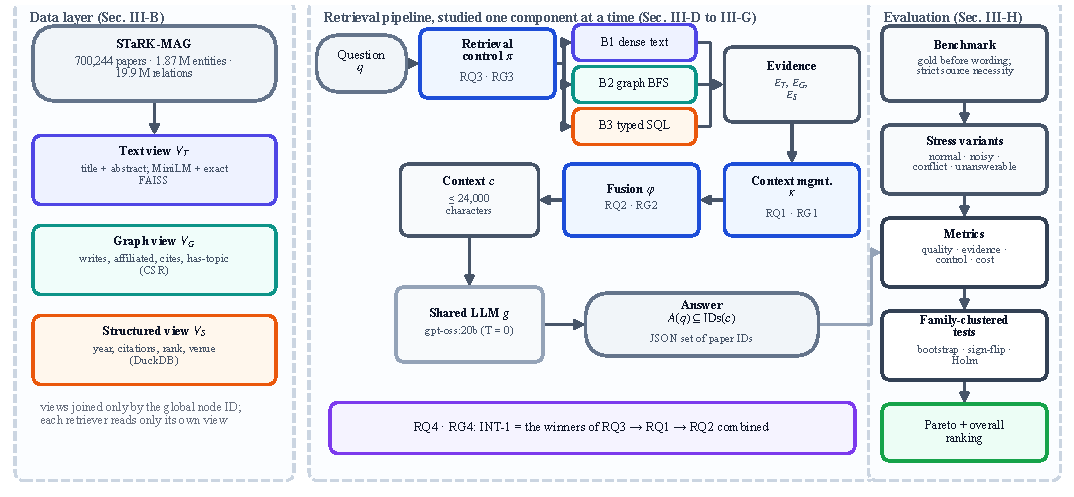
\includegraphics[width=\textwidth]{figures/fig_framework.pdf}
\caption{Overview of the controlled framework. Three isolated views of one corpus feed three fixed retrievers. Retrieval control (RQ3), context management of graph evidence (RQ1), and cross-modal fusion (RQ2) are studied one at a time under a shared language model; the best choice of each is then combined (RQ4). The evaluation layer computes quality and cost metrics and family-clustered paired tests.}
\label{fig:framework}
\end{figure*}

\begin{itemize}
\item \textbf{Isolated, identity-joined views.} Text, graph, and structured representations of the same 700,244 papers share nothing except the official node identifier, so any benefit of combining sources is a real benefit of combining them.
\item \textbf{Verified-by-construction benchmark.} Gold answers are computed from the frozen data before any question is worded; for every multi-source question, dropping any required source provably enlarges the answer set; noisy, conflicting, and unanswerable variants are added as evaluation-time overlays that never alter the canonical data.
\item \textbf{One variable at a time.} Fifteen strategies (nine adaptations of published methods and six simple controls) are compared under one frozen interface, and an integrated system is built by a selection rule fixed before any result was known.
\item \textbf{Replay-verified execution.} Every model request is stored under the hash of its full payload, and results are rebuilt by a runner that refuses to proceed if any request differs; the four studies (32, 24, 28, and 28 questions; 16 strategies) produced 448 run records with 0 errors.
\item \textbf{Correlation-aware statistics.} Paired differences are tested with family-clustered bootstrap intervals and exact sign-flip tests with Holm correction~\cite{holm1979,efron1993,cameron2008}, complemented by Pareto analysis and a transparent overall ranking.
\item \textbf{A clear, practical answer.} The simplest strategy wins every component on combined quality and cost, the integrated system inherits the router's significantly better source selection, and the dominant limitation is located upstream, in retrieval coverage.
\item \textbf{Open and inspectable.} All figures and tables are regenerated from checksummed study outputs, and an interactive application replays every recorded run step by step.
\end{itemize}

\subsection{Organization of the Paper}

Section~\ref{sec:lit} reviews related work, compares it with the problem studied here, and identifies the research gaps. Section~\ref{sec:method} formalizes the data, the pipeline, and every strategy, and describes how the problem was solved: the execution protocol, metrics, and statistics. Section~\ref{sec:results} reports and discusses the results. Section~\ref{sec:conclusion} concludes and lists limitations and future work, and Section~\ref{sec:availability} describes data and code availability.

\section{Literature Review}\label{sec:lit}

\subsection{Related Work}

\subsubsection{Retrieval-augmented generation}

RAG couples a retriever with a generator so that answers are conditioned on retrieved evidence~\cite{lewis2020}; surveys organize the many variants that followed~\cite{gao2023}. Two observations from this line of work motivate context management: models use long contexts unevenly, attending less to evidence in the middle of the input~\cite{liu2024lost}, and compressing or selecting evidence can reduce cost while preserving answers~\cite{jiang2024longllmlingua}. Active and self-reflective variants decide during generation whether and what to retrieve~\cite{jiang2023flare,asai2024selfrag}.

\subsubsection{Graph-based RAG}

GraphRAG systems retrieve entities, relations, and paths from a knowledge graph. GraphRAG~\cite{edge2024graphrag} builds an entity graph from text with an LLM and summarizes graph communities; G-Retriever~\cite{he2024gretriever} selects a compact subgraph with a prize-collecting Steiner tree~\cite{goemans1995,hegde2015pcst}; KG\textsuperscript{2}RAG~\cite{zhu2025kg2rag} expands semantically retrieved seeds through a knowledge graph and organizes them into connected, reranked paragraphs; QAFD-RAG~\cite{zhou2026qafd} lets relevance flow through the graph along query-aware edge weights, building on local flow diffusion~\cite{fountoulakis2020flow}; Think-on-Graph~\cite{sun2024tog} lets the LLM explore the graph by beam search; and HippoRAG~\cite{gutierrez2024hipporag} uses personalized graph propagation as long-term memory. A recent survey reviews the area~\cite{peng2024survey}.

\subsubsection{Fusion of heterogeneous knowledge}

Several systems combine unstructured and structured knowledge. UniK-QA~\cite{oguz2022unikqa} linearizes tables and knowledge-base triples into text; StructGPT~\cite{jiang2023structgpt} lets the LLM reason over structured interfaces; HybridRAG~\cite{sarmah2024hybridrag} concatenates vector and graph retrieval; KAG~\cite{liang2024kag} aligns knowledge-graph entities with source chunks through mutual indexing; SAG~\cite{wu2026sag} indexes events and entities in SQL and selects structural evidence at query time; MegaRAG~\cite{hsiao2025megarag} reasons over each modality before a final fusion stage; and query-driven multimodal GraphRAG~\cite{bu2025qdmm} builds local graphs on demand from text, tables, and images.

\subsubsection{Adaptive and agentic retrieval control}

Adaptive-RAG~\cite{jeong2024adaptive} trains a small classifier to route each question to no retrieval, single-step, or multi-step retrieval; CRAG~\cite{yan2024crag} scores retrieved evidence with a lightweight evaluator and triggers corrective actions; interleaved reasoning and retrieval~\cite{trivedi2023ircot} and reasoning-acting agents~\cite{yao2023react} decide the next retrieval step from intermediate reasoning; AGENT-G~\cite{agentg2025} equips an agent with a retriever bank and a critic of validator and commentor roles for hybrid textual and relational questions; and agent-orchestrated adaptive RAG~\cite{maharjan2026agent} adds decomposition and bounded reflection.

\subsubsection{Benchmarks and evaluation methodology}

STaRK~\cite{wu2024stark} evaluates retrieval over semi-structured knowledge bases, including an academic base derived from the Microsoft Academic Graph~\cite{wang2020mag}, which is the source corpus of this study. Methodological work in NLP stresses significance testing and the danger of treating dependent samples as independent~\cite{dror2018}; clustered resampling~\cite{cameron2008}, exact permutation tests~\cite{good2005}, and family-wise error control~\cite{holm1979} address these concerns.

\subsection{Comparison With the Current Research Problem}

Table~\ref{tab:lit} positions representative works with respect to the problem studied here: the component they address, the knowledge they use, their core mechanism, and their role in this study. The nine mechanisms marked in the last column are re-implemented as adaptations under one frozen interface (Sections III-D to III-F); the remaining works inform the design.

\begin{table*}[!t]
\caption{Representative related work and its relation to the present study}
\label{tab:lit}
\centering
\footnotesize
\setlength{\tabcolsep}{3pt}
\renewcommand{\arraystretch}{1.1}
\begin{tabular}{@{}>{\raggedright\arraybackslash}p{\dimexpr0.177\linewidth-2\tabcolsep\relax}>{\raggedright\arraybackslash}p{\dimexpr0.154\linewidth-2\tabcolsep\relax}>{\raggedright\arraybackslash}p{\dimexpr0.115\linewidth-2\tabcolsep\relax}>{\raggedright\arraybackslash}p{\dimexpr0.392\linewidth-2\tabcolsep\relax}>{\raggedright\arraybackslash}p{\dimexpr0.162\linewidth-2\tabcolsep\relax}@{}}
\toprule
\textbf{Work} & \textbf{Focus} & \textbf{Knowledge} & \textbf{Core mechanism} & \textbf{Role here} \\
\midrule
RAG~\cite{lewis2020} & retrieve and generate & text & dense retrieval conditioning a generator & baseline B1 \\
GraphRAG~\cite{edge2024graphrag} & graph construction & text $\rightarrow$ graph & LLM-extracted entity graph, community summaries & design input \\
G-Retriever~\cite{he2024gretriever} & context management & graph & prize-collecting Steiner tree subgraph (+ GNN soft prompt) & CM-02 \\
KG\textsuperscript{2}RAG~\cite{zhu2025kg2rag} & context management & text + graph & seed expansion, spanning-tree organization, reranking & CM-01 \\
QAFD-RAG~\cite{zhou2026qafd} & context management & graph & query-aware flow diffusion from keyword seeds & CM-03 \\
Think-on-Graph~\cite{sun2024tog} & retrieval control & graph & LLM beam search over the knowledge graph & design input \\
KAG~\cite{liang2024kag} & fusion & text + graph & mutual indexing, entity alignment, logical forms & CF-01 \\
SAG~\cite{wu2026sag} & fusion & text + structured & event--entity SQL index, query-time selection & CF-02 \\
MegaRAG~\cite{hsiao2025megarag} & fusion & text + graph + image & per-modality reasoning, then late fusion & CF-03 \\
QD multimodal GraphRAG~\cite{bu2025qdmm} & integrated & text, graph, table, image & query-driven local graph construction & design input \\
Adaptive-RAG~\cite{jeong2024adaptive} & retrieval control & text & complexity classifier routes retrieval depth & AR-01 \\
CRAG~\cite{yan2024crag} & retrieval control & text & retrieval evaluator triggers corrections & AR-02 \\
AGENT-G~\cite{agentg2025} & retrieval control & text + graph & agent, retriever bank, validator and commentor & AR-03 \\
STaRK~\cite{wu2024stark} & benchmark & text + relations & retrieval over semi-structured knowledge bases & source data \\
\textbf{This study} & \textbf{all three, then integration} & \textbf{text, graph, structured (isolated)} & \textbf{controlled comparison of 15 strategies + 1 integrated system} & --- \\
\bottomrule
\end{tabular}
\end{table*}

The comparison exposes the gap between these works and the research problem. Each mechanism was proposed for a different combination of sources and evaluated inside its own system, so the literature offers many candidate answers to RQ1--RQ3 but no common ground on which to compare them. The problem studied here requires (i) the three knowledge forms to be available as separate sources over the same entities, (ii) questions whose answers provably need several sources, (iii) every candidate strategy to run against identical evidence, retrievers, model, prompt, and budget, and (iv) quality and cost to be judged together with statistics suited to small, correlated question sets.

\subsection{Review Outcome}

The review leads to four outcomes (RO).

\begin{itemize}
\item \textbf{RO1. Effects are not attributable.} Mechanisms for the three components are evaluated inside different systems with different corpora, retrievers, models, prompts, and budgets; reported gains cannot be attributed to one component or compared across papers.
\item \textbf{RO2. Sources are often entangled.} When a graph is extracted from the same text that is also retrieved, graph and text evidence overlap, and the value of each representation is confounded.
\item \textbf{RO3. Multi-source questions are rarely verified.} Benchmarks seldom guarantee that every listed source is necessary for a question, and robustness to distractors, conflicting facts, and unanswerable questions is seldom tested together with source necessity.
\item \textbf{RO4. Cost and uncertainty are under-reported.} Elaborate controllers add model calls and tokens, yet quality is often reported without cost, and small sets of related question variants call for correlation-aware significance testing~\cite{dror2018}.
\end{itemize}

\subsection{Problem Identification}

The review outcomes translate into four research gaps (RG), one per research question (Table~\ref{tab:gaps}). RG1--RG3 concern the three pipeline components and RG4 their combination; the methods that address them are presented in Sections III-D to III-G.

\begin{table}[!t]
\caption{Research gaps derived from the review and how they are addressed}
\label{tab:gaps}
\centering
\footnotesize
\setlength{\tabcolsep}{3pt}
\renewcommand{\arraystretch}{1.1}
\begin{tabular}{@{}>{\raggedright\arraybackslash}p{\dimexpr0.183\linewidth-2\tabcolsep\relax}>{\raggedright\arraybackslash}p{\dimexpr0.583\linewidth-2\tabcolsep\relax}>{\raggedright\arraybackslash}p{\dimexpr0.233\linewidth-2\tabcolsep\relax}@{}}
\toprule
\textbf{Gap} & \textbf{Description} & \textbf{Addressed by} \\
\midrule
RG1 & No controlled comparison of graph-context strategies under a fixed budget with identical evidence & RQ1, Section~\ref{sec:cm} \\
RG2 & No controlled comparison of fusion strategies on byte-identical multi-source evidence & RQ2, Section~\ref{sec:cf} \\
RG3 & No controlled comparison of source-selection policies with the same retrievers and context format & RQ3, Section~\ref{sec:ar} \\
RG4 & Unknown combined effect of empirically chosen components & RQ4, Section~\ref{sec:int} \\
\bottomrule
\end{tabular}
\end{table}

\textbf{Problem statement.} Let a corpus offer a text view, a graph view, and a structured view of the same papers, joined only by a global identifier. Each question $q$ has a verified answer set $G(q)$ of paper identifiers, possibly empty. A system queries some of the views, builds a context within a fixed budget, and asks a fixed LLM for an answer set $A(q)$ that may only contain identifiers present in the context. For each component in turn, with all others held fixed, find the strategy that makes $A(q)$ match $G(q)$ most closely while keeping cost (tokens, model calls, searches, latency) low; accept a difference only when a paired, correlation-aware test supports it; and finally measure the combination of the chosen strategies.

Fig.~\ref{fig:example} illustrates why such questions are hard. In a validation question requiring all three sources, each source alone admits between 111 and 130,859 papers, while exactly one paper satisfies all conditions; removing any single source admits between 1 and 151 wrong papers.

\begin{figure}[!t]
\centering
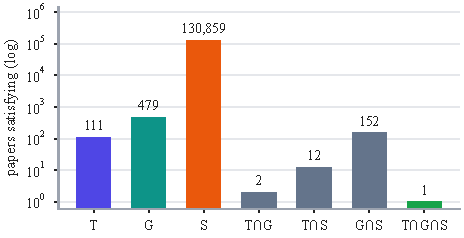
\includegraphics[width=0.94\columnwidth]{figures/fig_example.pdf}
\caption{Candidate papers that satisfy the conditions of one three-source benchmark question, per source and per intersection (log scale). Only the paper in the triple intersection is correct; every source is necessary.}
\label{fig:example}
\end{figure}

\section{Method}\label{sec:method}

\subsection{Overview: What Is Studied and How}\label{sec:overview}

\emph{What} is studied are the three components of a multi-source RAG pipeline (retrieval control, context management, and fusion) and their combination. \emph{How} they are studied is a controlled protocol: in each study exactly one component varies across five strategies while the data, retrievers, LLM, prompt, and budget stay fixed; the study is frozen by checksum before it runs; every model call is stored and replay-verified; and differences are tested with paired, family-clustered statistics. We write T, G, and S for the text, graph, and structured sources and TG, TS, GS, and TGS for the combinations that a question requires. Table~\ref{tab:design} lists the four study designs.

\subsection{Data Modeling}\label{sec:data}

\subsubsection{Three isolated views}

Let $\mathcal{N}$ be the set of entities of STaRK-MAG~\cite{wu2024stark,wang2020mag}, each with a global identifier, and $\mathcal{P}\subset \mathcal{N}$ its papers. The \textbf{text view} $V_T$ holds one document per paper, the exact title followed by the abstract, embedded with a frozen MiniLM sentence encoder~\cite{reimers2019sbert,wang2020minilm} (384 dimensions, 256-token input) and indexed exactly with FAISS~\cite{johnson2021faiss}. The \textbf{graph view} $V_G=(\mathcal{N},\mathcal{E})$ holds the four official relation types (writes, affiliated-with, cites, has-topic), where a paper's label is its title only; each of the 19,919,698 directed edges also receives a tagged inverse row for traversal, stored as memory-mapped compressed sparse rows. The \textbf{structured view} $V_S$ is a DuckDB table~\cite{raasveldt2019duckdb} of nullable paper attributes (year, date, citation count, rank, venue, document type), in which missing values remain NULL. The views share nothing except the identifier: the text view contains no authors, years, or venues, the graph view contains no abstracts or attributes, and the structured view contains no text or relations. Table~\ref{tab:data} summarizes the corpus and the benchmark.

\subsubsection{Verified multi-source questions}

Each generated question $q$ requires a set of sources $M(q)\subseteq \{T,G,S\}$. For each required source $m$, a condition is evaluated on the frozen view before any wording, giving a candidate set $C_m (q)$: an exact abstract phrase for text, an authorship, affiliation, or citation path for the graph, and parameterized predicates for structured data. The gold set is their intersection,
\begin{equation}
G(q)=\bigcap_{m\in M(q)} C_m(q)
\label{eq:gold}
\end{equation}
and every multi-source question must satisfy \textbf{strict source necessity}:
\begin{equation}
\forall m\in M(q):\quad G_{-m}(q)=\bigcap_{m'\in M(q)\setminus\{m\}} C_{m'}(q)\supsetneq G(q)
\label{eq:necessity}
\end{equation}

Questions are worded from templates and never contain an answer identifier or title. Each base question has up to four \textbf{variants}: normal; \emph{noisy}, which adds hard distractors that fail one condition; \emph{conflict}, which adds one altered fact about a correct paper while the canonical record stays authoritative; and \emph{unanswerable}, which adds a provably disjoint condition so that $G(q)=\emptyset$. The variants of one base question form a \textbf{family}, the independent unit of all statistics. Algorithm~\ref{alg:bench} summarizes the construction; an independent audit recomputed every gold set, all 665,671 candidate identifiers, and all 2,336 witness paths, and a full regeneration reproduced all benchmark files byte for byte.

\begin{table*}[!t]
\caption{Design of the four studies (all questions are programmatically verified validation questions)}
\label{tab:design}
\centering
\footnotesize
\setlength{\tabcolsep}{3pt}
\renewcommand{\arraystretch}{1.1}
\begin{tabular}{@{}>{\raggedright\arraybackslash}p{\dimexpr0.073\linewidth-2\tabcolsep\relax}>{\raggedright\arraybackslash}p{\dimexpr0.220\linewidth-2\tabcolsep\relax}>{\raggedright\arraybackslash}p{\dimexpr0.207\linewidth-2\tabcolsep\relax}>{\raggedright\arraybackslash}p{\dimexpr0.287\linewidth-2\tabcolsep\relax}>{\raggedright\arraybackslash}p{\dimexpr0.213\linewidth-2\tabcolsep\relax}@{}}
\toprule
\textbf{Study} & \textbf{Cohort} & \textbf{What changes} & \textbf{What stays fixed} & \textbf{Metrics} \\
\midrule
RQ1 & 32 questions: 8 families (2 each for G, TG, GS, TGS) $\times$ 4 variants (normal, noisy, conflict, unanswerable) & selection, order, and pruning of graph evidence & graph candidate pool; text and structured evidence passed through; LLM; prompt; 24,000-character budget & F1 (primary); MRR, gold coverage, tokens, latency \\
RQ2 & 24 frozen bundles: 8 families (2 each for TG, TS, GS, TGS) $\times$ 3 variants (normal, noisy, conflict) & combination of text, graph, structured evidence & byte-identical bundles, no retrieval; LLM; prompt; 24,000-character budget & F1 (primary); EM, MRR, model calls, tokens, latency \\
RQ3 & 28 questions: 14 families (2 for each of the 7 source combinations) $\times$ 2 variants (normal, noisy) & which source, in which order, when to stop & retrievers B1--B3; 8,000 characters per queried source; LLM; prompt & F1 (primary); source-selection F1, wasted retrieval, stopping accuracy, calls, tokens, latency \\
RQ4 & the 28 questions of RQ3 & combination of the selected components & questions, data, retrievers, LLM, prompt & F1 (primary); source-selection F1, tokens, latency \\
\bottomrule
\end{tabular}
\end{table*}

\begin{table}[!t]
\caption{Corpus (MMG-STaRK-MAG) and benchmark statistics}
\label{tab:data}
\centering
\footnotesize
\setlength{\tabcolsep}{3pt}
\renewcommand{\arraystretch}{1.1}
\begin{tabular}{@{}>{\raggedright\arraybackslash}p{\dimexpr0.517\linewidth-2\tabcolsep\relax}>{\raggedleft\arraybackslash}p{\dimexpr0.483\linewidth-2\tabcolsep\relax}@{}}
\toprule
\textbf{Item} & \textbf{Value} \\
\midrule
Papers / authors & 700,244 / 1,104,554 \\
Institutions / fields of study & 8,701 / 59,469 \\
Official directed relations & 19,919,698 \\
writes / affiliated / cites / has-topic & 6.77 M / 1.03 M / 4.88 M / 7.24 M \\
Graph traversal rows (with tagged inverses) & 39,839,396 \\
Structured rows / with missing attributes & 700,244 / 22,049 \\
Benchmark questions & 13,571 \\
train / validation / test / human test & 8,049 / 2,721 / 2,720 / 81 \\
Generated, verified questions & 167 \\
Validation families used & 14 (7 combinations $\times$ 2) \\
\bottomrule
\end{tabular}
\end{table}

\subsection{Retrieval and Generation Model}\label{sec:pipeline}

All strategies share three deliberately simple retrievers, each returning its top five results. \textbf{B1} embeds the question and returns the five most similar papers from the exact FAISS index. \textbf{B2} resolves up to three seed entities from graph labels and traverses breadth-first to depth 2 under fixed caps (2,000 nodes, 20,000 scanned edges, 128 edges per node), returning the five best-ranked papers with their paths. \textbf{B3} parses supported conditions into a typed conjunctive plan compiled into parameterized, read-only SQL. A fourth baseline, \textbf{B4}, runs all three and writes their evidence in fixed sections. None of them reranks, rewrites queries, or falls back to another source.

\begin{algorithm}[!t]
\caption{Verified multi-source question construction}
\label{alg:bench}
\begin{algorithmic}[1]
\Require frozen views $V_T,V_G,V_S$; source combination $M$; split; seed 42
\Ensure question $q$, gold set $G(q)$, stress variants
\State choose one condition per $m\in M$ from split-exclusive anchors
\State \textbf{for each} $m\in M$ \textbf{do} compute $C_m (q)$ on the frozen view (sorted, hashed)
\State $G(q)\leftarrow \bigcap _m C_m (q)$
\State \textbf{for each} $m\in M$ \textbf{with} $|M|>1$ \textbf{do}
\State \hspace*{1\algorithmicindent}\textbf{if} $G_{-m} (q)=G(q)$ \textbf{then reject} the construction \textbf{else} store counter-examples
\State word $q$ from a template (no answer identifiers or titles)
\State add overlays: noisy distractors, one conflicting fact, one disjoint condition ($G=\emptyset$)
\State recompute all sets independently; regenerate and compare bytes
\State \textbf{return} $q$, $G(q)$, variants
\end{algorithmic}
\end{algorithm}

Writing $\pi$ for the retrieval-control policy, $\kappa$ for context management of graph evidence, $\varphi$ for fusion, and $g$ for the LLM, a question is answered as
\begin{equation}
A(q)=g\bigl(q,\varphi(E_T,\kappa(E_G),E_S)\bigr),\quad E=\bigcup_{t=1}^{k}\mathcal{R}_{s_t}(q_t)
\label{eq:pipeline}
\end{equation}
where $\pi$ chooses the source $s_t$ and query $q_t$ of each step $t$ and the number of steps $k$, and the evidence of each source is collected in $E_T$, $E_G$, and $E_S$. The serialized context must satisfy $|{\text{ser}}(c)|\le B$, with $B$ = 24,000 characters. The LLM is \textbf{gpt-oss:20b}~\cite{openai2025gptoss}, served locally by Ollama 0.40.5~\cite{ollama} with temperature 0, a per-question seed, low reasoning effort, JSON output, and a 1,024-token completion cap for every call. A single grounding prompt instructs it to answer only from the evidence, to require every condition, to treat NULL as unknown, and to prefer canonical records over tagged overlays. A strict parser accepts only integer paper identifiers present in the context; anything else is recorded as a failure, and an empty set is a valid abstention.

\subsection{RG1 $\rightarrow$ RQ1: Context Management Strategies}\label{sec:cm}

Context management decides which graph evidence reaches the model. All five strategies receive the same bounded candidate pool per question (a depth-2 neighbourhood of B2's seeds with at most 256 base nodes and 1,024 base edges), and text and structured evidence pass through unchanged. Fig.~\ref{fig:cm} illustrates the five strategies on a toy graph.

\begin{figure*}[!t]
\centering
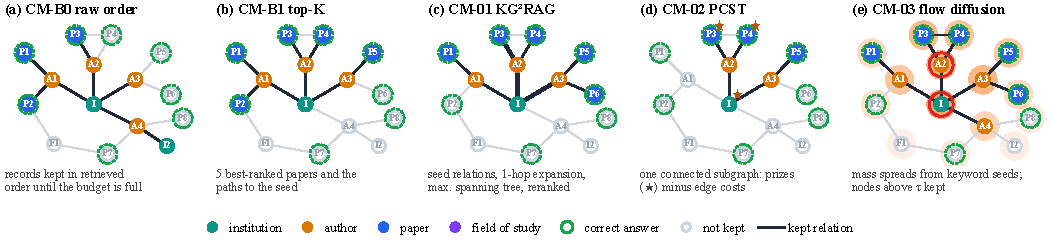
\includegraphics[width=\textwidth]{figures/fig_rq1_methods.pdf}
\caption{The five context-management strategies of RQ1 on a schematic candidate graph for the question ``papers with an author affiliated with institution I''. Filled nodes and dark edges are kept in the context. (a) Raw order keeps records until the budget is full. (b) Fixed top-K keeps the five best-ranked papers and their paths. (c) KG\textsuperscript{2}RAG-inspired: seed relations, one-hop expansion, and maximum spanning trees (thick edges), reranked. (d) PCST-inspired: one connected subgraph trading prizes ($\bigstar$) against edge costs. (e) Flow diffusion: mass spreads from keyword seeds (red rings); nodes above a threshold are kept.}
\label{fig:cm}
\end{figure*}

\textbf{CM-B0 (raw order)} writes node and edge records in candidate order and stops at the first record that does not fit. \textbf{CM-B1 (fixed top-K)} keeps the first five papers in retriever order (path length, seed rank, identifier) together with the parent paths that connect them to their seeds, serialized depth-first.

\textbf{CM-01 (KG\textsuperscript{2}RAG-inspired)}~\cite{zhu2025kg2rag}. The original links text chunks to the graph triples extracted from them; STaRK provides no such provenance, so we use \emph{graph-native provenance units}: one sentence per official relation, written from labels and identifiers only (e.g., ``Author \emph{a} writes Paper \emph{p}.''). With MiniLM embeddings $\mathbf{h}$, each unit $u_e$ of edge $e$ is weighted by its similarity $w(e)=\cos(\mathbf{h}_q,\mathbf{h}_{u_e})$ to the question, the ten best units become seeds, the graph is expanded by one hop inside the pool, and each connected component $K_k$ is organized as a maximum spanning tree computed with Kruskal's algorithm~\cite{kruskal1956}:
\begin{equation}
T_k=\operatorname*{arg\,max}_{T\in\mathcal{T}(K_k)}\sum_{e\in T} w(e)
\label{eq:mst}
\end{equation}

Each tree is written depth-first from its highest-weight edge, scored with a BGE cross-encoder reranker~\cite{xiao2024cpack}, deduplicated, and packed into the budget in rank order (Algorithm~\ref{alg:cm01}).

\textbf{CM-02 (G-Retriever-inspired)}~\cite{he2024gretriever}. The three nodes and five edges most similar to the question receive rank prizes $\pi$ (3, 2, 1 and 5 to 1); every edge costs $c_e=0.5$; and the prize-collecting Steiner tree problem~\cite{goemans1995}
\begin{equation}
T^*=\operatorname*{arg\,min}_{T}\Bigl(\sum_{e\in E(T)} c_e+\sum_{v\notin V(T)}\pi_v\Bigr)
\label{eq:pcst}
\end{equation}
is solved with the pcst\_fast solver~\cite{hegde2015pcst} (unrooted, one tree, edge prizes via virtual nodes). The resulting connected subgraph is written breadth-first and trimmed leaf by leaf to the budget. The original's graph neural network and soft prompt are omitted.

\begin{algorithm}[!t]
\caption{CM-01 graph-native KG\textsuperscript{2}RAG context construction}
\label{alg:cm01}
\begin{algorithmic}[1]
\Require question $q$, candidate pool $(\mathcal{V},\mathcal{E})$, budget $B_G$
\Ensure graph context
\State build one provenance unit $u_e$ per official edge $e\in \mathcal{E}$ (labels and identifiers only)
\State score $w(e)=\cos(\mathbf{h}_q,\mathbf{h}_{u_e})$; seeds $\leftarrow$ the 10 best units
\State expand one hop around the seeds inside the pool
\State \textbf{for each} connected component $K_k$ \textbf{do}
\State \hspace*{1\algorithmicindent}$T_k\leftarrow$ maximum spanning tree of $K_k$ under $w$ (Kruskal; ties by unit ID)
\State \hspace*{1\algorithmicindent}serialize $T_k$ depth-first from its highest-weight edge
\State rank the trees with the cross-encoder; remove duplicate units
\State \textbf{return} trees in rank order while they fit in $B_G$
\end{algorithmic}
\end{algorithm}

\textbf{CM-03 (QAFD-RAG-inspired)}~\cite{zhou2026qafd}. One LLM call extracts the question's keywords; the 20 nodes most similar to any keyword become seeds with mass 10 each. With the non-negative cosine similarity
\begin{equation}
H(a,b)=\frac{1+\cos(\mathbf{h}_a,\mathbf{h}_b)}{2}
\label{eq:hsim}
\end{equation}
mass is pushed along edges with query-aware conductance
\begin{equation}
w(u,v)=H(u,v)\Bigl(1+\frac{1}{4}\bigl(H(u,q)+H(v,q)\bigr)\Bigr)
\label{eq:conductance}
\end{equation}
where every node can retain at most one unit of mass (sink capacity), following local flow diffusion~\cite{fountoulakis2020flow}. Diffusion stops when the total excess is at most $\varepsilon =0.05$ or after $10^6$ pushes. With the excess and the support
\begin{equation}
\mathrm{ex}(v)=\max(0,x_v-1),\quad \mathcal{S}=\{v: x_v>\tau\}
\label{eq:support}
\end{equation}
for $\tau =0.01$, the support plus the connectors between its nodes is pruned from the outside in until it fits (Algorithm~\ref{alg:cm03}).

\subsection{RG2 $\rightarrow$ RQ2: Cross-Modal Fusion Strategies}\label{sec:cf}

Fusion decides how the three evidence streams are presented. To isolate it completely, every method receives the \textbf{byte-identical cached evidence bundle} of each question (the top-5 evidence of B1, B2, and B3 plus the variant's overlays) and may not retrieve. Fig.~\ref{fig:cf} contrasts the context layouts.

\begin{figure*}[!t]
\centering
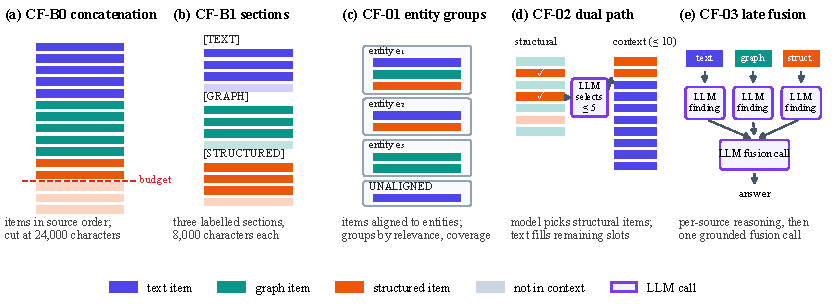
\includegraphics[width=\textwidth]{figures/fig_rq2_methods.pdf}
\caption{Context layouts of the five fusion strategies of RQ2 on the same evidence bundle. (a) Raw concatenation in source order, cut at the budget. (b) Three labelled sections with a third of the budget each. (c) Evidence grouped by aligned entity. (d) An LLM selects up to five structural items; text fills the remaining slots. (e) One reasoning call per source, then a grounded fusion call.}
\label{fig:cf}
\end{figure*}

\begin{algorithm}[!t]
\caption{CM-03 query-aware flow diffusion}
\label{alg:cm03}
\begin{algorithmic}[1]
\Require question $q$, candidate pool, budget $B_G$
\Ensure graph context
\State keywords $\leftarrow$ LLM($q$) (one call, strict JSON)
\State seeds $\leftarrow$ 20 nodes with the highest keyword similarity; $x_v\leftarrow 10$ for each seed
\State \textbf{while} $\sum _v {\text{ex}}(v)>\varepsilon$ \textbf{and} pushes $<10^6$ \textbf{do}
\State \hspace*{1\algorithmicindent}$v\leftarrow$ node with the largest excess (ties by ID)
\State \hspace*{1\algorithmicindent}push ${\text{ex}}(v)$ to neighbours in proportion to $w(v,u)$ from \eqref{eq:conductance}
\State $\mathcal{S}\leftarrow \{v:x_v>\tau \}$ plus connector nodes
\State prune the lowest-mass outer nodes of $\mathcal{S}$ until it fits $B_G$
\State \textbf{return} serialized $\mathcal{S}$
\end{algorithmic}
\end{algorithm}

\textbf{CF-B0 (raw concatenation)} writes all items in source order until the budget is reached. \textbf{CF-B1 (source-separated)} writes labelled TEXT, GRAPH, and STRUCTURED sections, each limited to 8,000 characters.

\textbf{CF-01 (KAG-inspired entity alignment)}~\cite{liang2024kag} attaches every evidence item to an entity in a fixed order (explicit identifier, then a unique exact normalized alias, then a registry lookup restricted to the item's entity type); unresolved items form UNALIGNED groups. Groups are ordered by their best member relevance, then by the number of sources they cover, then by entity identifier, and written whole until the budget is full. No model invents entities.

\textbf{CF-02 (SAG-inspired dual path)}~\cite{wu2026sag} treats graph and structured items as \emph{structural} and text items as \emph{semantic} candidates. One selector call reads a compact manifest of the structural candidates (one line each: identifier, source, relevance, the first 200 characters, provenance) and returns at most five identifiers; one schema repair is allowed, otherwise the five most relevant items are used. Text items then fill the context to ten items in retriever order.

\textbf{CF-03 (MegaRAG-inspired late fusion)}~\cite{hsiao2025megarag} reasons over each non-empty source separately and fuses the findings (Algorithm~\ref{alg:cf03}).

\begin{algorithm}[!t]
\caption{CF-03 late fusion with grounded findings}
\label{alg:cf03}
\begin{algorithmic}[1]
\Require question $q$, bundle with sources $\{T,G,S\}$
\Ensure answer $A(q)$
\State \textbf{for each} source $s$ with evidence \textbf{do}
\State \hspace*{1\algorithmicindent}$f_s\leftarrow$ LLM($q$, evidence of $s$ only) as \{candidate\_answer, supporting\_ids, confidence\}
\State \hspace*{1\algorithmicindent}\textbf{if} supporting\_ids $\not\subseteq$ IDs($s$) \textbf{or} the call fails \textbf{then} $f_s\leftarrow$ NO\_EVIDENCE
\State $A(q)\leftarrow$ LLM($q$, $\{f_s\}$), citing only papers supported by some $f_s$
\State \textbf{if} the fusion call fails \textbf{then} retry once, \textbf{else return} $A(q)$
\end{algorithmic}
\end{algorithm}

Fusion cannot recover evidence that was never retrieved. Before any model call, each bundle $b$ with evidence papers $P(b)$ was therefore assigned a supportability class, used only for analysis:
\begin{equation}
\mathrm{class}(b)=\begin{cases}\text{FULLY} & \text{if } G(q)\subseteq P(b)\\ \text{PARTIALLY} & \text{if } G(q)\cap P(b)\neq\emptyset\\ \text{UNSUPPORTABLE} & \text{otherwise}\end{cases}
\label{eq:supp}
\end{equation}

\subsection{RG3 $\rightarrow$ RQ3: Retrieval-Control Policies}\label{sec:ar}

Retrieval control decides which sources to query, in which order, and when to stop. All policies share the same tools (the unchanged B1--B3), a cumulative evidence memory, and a fixed downstream context (labelled sections of 8,000 characters for the sources actually queried), so the policy is the only variable. Fig.~\ref{fig:ar} shows their control flow.

\textbf{AR-B0} always queries text, graph, and structured with the raw question. \textbf{AR-B1 (rule router)} normalizes the question (NFKC, lowercase) and matches a frozen cue table: text cues (e.g., ``abstract'', ``mentions''), graph cues (e.g., ``author'', ``affiliated'', ``cites''), and structured cues (e.g., ``year'', ``rank'', ``at least'', ``$\ge$''). It queries every matched source once in the order text, graph, structured; with no match it queries text. The cue table was frozen before any result and serves as the base router of AR-01 and AR-02.

\begin{figure*}[!t]
\centering
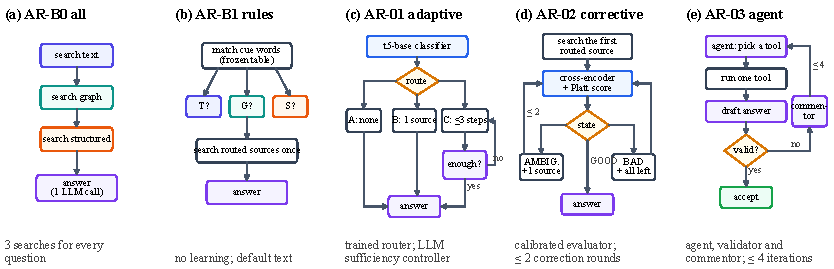
\includegraphics[width=\textwidth]{figures/fig_rq3_methods.pdf}
\caption{Control flow of the five retrieval-control policies of RQ3. (a) Always query all three sources. (b) Frozen keyword cues select the sources. (c) A trained classifier chooses no retrieval, one source, or multi-step retrieval with an LLM sufficiency check. (d) A calibrated cross-encoder rates the evidence and triggers corrections. (e) An agent chooses one tool per step; a validator accepts or a commentor returns feedback.}
\label{fig:ar}
\end{figure*}

\textbf{AR-01 (Adaptive-RAG-inspired)}~\cite{jeong2024adaptive}. A t5-base model~\cite{raffel2020t5} predicts a route: A (no retrieval), B (the router's first source), or C (up to three steps, with an LLM controller returning \{sufficient, next\_subquery\} after each step). Training labels come from a retrieval-only oracle on separate training questions:
\begin{equation}
\ell(q)=\min\{\ell\in(A,B,C):\mathrm{succ}_\ell(q)\}
\label{eq:label}
\end{equation}
where A succeeds only for an empty gold set, B succeeds if the router's first source retrieves every gold paper, and C if up to three sources do; the label defaults to C. A hash-based partition of the 8,049 training questions gave 7,302 training and 747 development questions; the model (AdamW, learning rate $3\times 10^{-5}$, weight decay 0.01) kept the epoch with the lowest development loss (epoch 7, loss 0.2170).

\textbf{AR-02 (CRAG-inspired)}~\cite{yan2024crag}. A MiniLM cross-encoder trained on MS MARCO~\cite{nogueira2019monobert,bajaj2016msmarco} scores each (question, evidence) pair; Platt scaling~\cite{platt1999}, fitted on the development partition only (7,498 labelled items from 745 questions), maps a raw score $s$ to a probability
\begin{equation}
p=\frac{1}{1+e^{-(as+b)}},\quad a=0.376,\quad b=0.102
\label{eq:platt}
\end{equation}
and the evidence state follows
\begin{equation}
\mathrm{state}(q)=\begin{cases}\text{GOOD} & \text{if } \max_i p_i\ge U\\ \text{BAD} & \text{if } \max_i p_i\le L\\ \text{AMBIGUOUS} & \text{otherwise}\end{cases}
\label{eq:state}
\end{equation}
with $L=0.40$ and $U=0.75$ chosen by macro-F1 from a frozen grid on 2,235 development states (Algorithm~\ref{alg:ar02}).

\textbf{AR-03 (AGENT-G-inspired)}~\cite{agentg2025}. An LLM agent chooses one action per iteration (a source with a query, or stop); after each tool call a candidate answer is generated and an LLM validator, which never sees gold data, accepts or rejects it; on rejection an LLM commentor returns feedback (Algorithm~\ref{alg:ar03}).

\begin{algorithm}[!t]
\caption{AR-02 calibrated corrective retrieval}
\label{alg:ar02}
\begin{algorithmic}[1]
\Require question $q$; router order; thresholds $L,U$
\Ensure answer $A(q)$
\State query the router's first source; rounds $\leftarrow 0$
\State \textbf{loop}
\State \hspace*{1\algorithmicindent}$p_i\leftarrow$ Platt(cross-encoder($q$, item $i$)) for all items; state by \eqref{eq:state}
\State \hspace*{1\algorithmicindent}\textbf{if} state = GOOD \textbf{or} rounds = 2 \textbf{or} no source is left \textbf{then break}
\State \hspace*{1\algorithmicindent}\textbf{if} AMBIGUOUS \textbf{then} add the next unqueried source \textbf{else} add all remaining
\State \hspace*{1\algorithmicindent}rounds $\leftarrow$ rounds + 1
\State \textbf{return} $g(q,{\text{fixed context}})$
\end{algorithmic}
\end{algorithm}

\begin{algorithm}[!t]
\caption{AR-03 agent--validator--commentor loop}
\label{alg:ar03}
\begin{algorithmic}[1]
\Require question $q$; at most $T=4$ iterations
\Ensure answer $A(q)$ or INSUFFICIENT\_EVIDENCE
\State \textbf{for} $i=1,\ldots ,T$ \textbf{do}
\State \hspace*{1\algorithmicindent}action $\leftarrow$ agent($q$, feedback, memory) (one schema repair allowed)
\State \hspace*{1\algorithmicindent}\textbf{if} action = stop \textbf{then return} $g(q,{\text{memory}})$
\State \hspace*{1\algorithmicindent}run exactly one tool; add new evidence to memory
\State \hspace*{1\algorithmicindent}$\hat{A}\leftarrow g(q,{\text{memory}})$; verdict $\leftarrow$ validator($q$, $\hat{A}$, memory)
\State \hspace*{1\algorithmicindent}\textbf{if} verdict accepts \textbf{then return} $\hat{A}$
\State \hspace*{1\algorithmicindent}feedback $\leftarrow$ commentor($q$, action, verdict); stop on repeated empty actions
\State \textbf{return} INSUFFICIENT\_EVIDENCE (empty answer)
\end{algorithmic}
\end{algorithm}

\subsection{RG4 $\rightarrow$ RQ4: Integration}\label{sec:int}

The integrated system \textbf{INT-1} chains the selected policy, context management on graph evidence, and the selected fusion method, whose answer becomes the system's answer. The components were selected by rules fixed before any RQ2 or RQ3 result was analysed: context management was fixed to CM-B1 for cost, and the policy and fusion method are the Pareto-optimal strategies with the highest answer F1,
\begin{equation}
m^*=\operatorname*{arg\,max}_{m\in\mathcal{P}} F_1(m)
\label{eq:select}
\end{equation}
with ties broken by fewer tokens and then by a fixed order. INT-1 is compared with AR-B0 and with the selected policy alone on the same 28 questions.

\subsection{How the Problem Was Solved: Execution and Evaluation Protocol}\label{sec:protocol}

\subsubsection{Freezing and replay-verified execution}

Before a study runs, its execution plan records the SHA-256 of every code file, configuration, prompt, input file, model artefact, and the exact cohort; a runner refuses to start or resume if any hash differs. Every model request is stored durably under the hash of its full payload. Calls are made question by question for all methods (question-major order), after which the unchanged evaluation runner replays each method with a store-only client that stops on any request that differs from the stored one (Fig.~\ref{fig:protocol}). Failures are recorded, never silently retried.

\begin{figure}[!t]
\centering
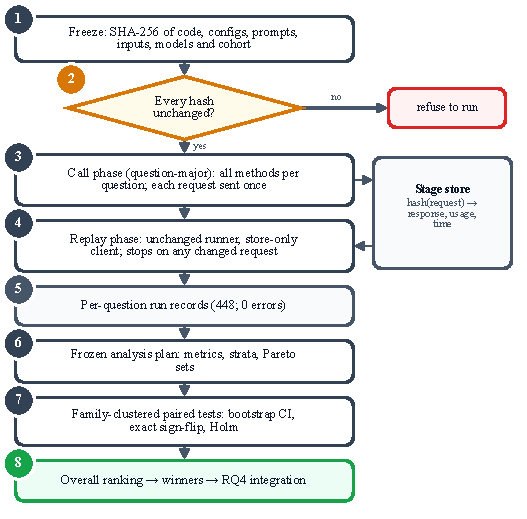
\includegraphics[width=0.94\columnwidth]{figures/fig_protocol.pdf}
\caption{Execution and analysis protocol: freeze, verify, call once per request in question-major order, replay with a byte-identity check, then analyse with a frozen plan.}
\label{fig:protocol}
\end{figure}

\subsubsection{Metrics}

For a question with returned set $A$ and gold set $G$,
\begin{equation}
P=\frac{|A\cap G|}{|A|},\quad R=\frac{|A\cap G|}{|G|},\quad F_1=\frac{2PR}{P+R}
\label{eq:prf}
\end{equation}
with the conventions that an empty prediction for an empty gold set scores 1 and an empty prediction for a non-empty gold set scores 0; exact match is $\mathbb{I}[A=G]$. Evidence quality is measured by the mean reciprocal rank of the first correct paper and by gold coverage, the share of correct papers present in the model's context:
\begin{equation}
\mathrm{GC}(q)=\frac{|G(q)\cap\mathrm{IDs}(c(q))|}{|G(q)|}
\label{eq:gc}
\end{equation}

For retrieval control, with $S$ the set of queried sources and $R$ the sources a question requires (known from its construction and used only for evaluation),
\begin{equation}
\mathrm{SF}_1=\frac{2|S\cap R|}{|S|+|R|},\quad \mathrm{WR}=\frac{|S\setminus R|}{|S|}
\label{eq:source}
\end{equation}
and stopping accuracy is 1 when the policy stops exactly at the first step after which all required sources have been queried. Cost is measured by input and output tokens over all model calls, model and retrieval calls, and intrinsic latency $L=t_{\text{ret}}+t_{\text{LLM}}+t_{\text{loc}}$ (retrieval time, model compute time, and local computation; waiting is excluded). Table~\ref{tab:metrics} summarizes the metrics.

\begin{table}[!t]
\caption{Metrics ($\uparrow$ higher is better, $\downarrow$ lower is better)}
\label{tab:metrics}
\centering
\footnotesize
\setlength{\tabcolsep}{3pt}
\renewcommand{\arraystretch}{1.1}
\begin{tabular}{@{}>{\raggedright\arraybackslash}p{\dimexpr0.306\linewidth-2\tabcolsep\relax}>{\raggedright\arraybackslash}p{\dimexpr0.597\linewidth-2\tabcolsep\relax}>{\centering\arraybackslash}p{\dimexpr0.097\linewidth-2\tabcolsep\relax}@{}}
\toprule
\textbf{Metric} & \textbf{Definition} & \textbf{} \\
\midrule
Answer F1 & set F1 of returned vs. gold papers, \eqref{eq:prf} & $\uparrow$ \\
Exact match (EM) & returned set equals gold set & $\uparrow$ \\
MRR & reciprocal rank of first correct paper & $\uparrow$ \\
Gold coverage (GC) & share of gold papers in the context, \eqref{eq:gc} & $\uparrow$ \\
Source F1 (SF1) & F1 of queried vs. required sources, \eqref{eq:source} & $\uparrow$ \\
Wasted retrieval (WR) & share of queried sources not needed, \eqref{eq:source} & $\downarrow$ \\
Stopping accuracy & stopped exactly when all needed sources were in hand & $\uparrow$ \\
Tokens & input + output tokens over all model calls & $\downarrow$ \\
Calls / searches & model calls / retriever calls per question & $\downarrow$ \\
Latency & retrieval + model compute + local time & $\downarrow$ \\
\bottomrule
\end{tabular}
\end{table}

\subsubsection{Statistical analysis}

For a pair of methods (A, B) and a metric, let $d(q)$ be the per-question difference, $S_f$ its sum over the questions of family $f$, and $n_f$ their number. Confidence intervals come from a family bootstrap~\cite{efron1993,cameron2008} with 10,000 resamples (seed 42):
\begin{equation}
\hat{\Delta}_b=\frac{\sum_{f\in\mathcal{B}_b} S_f}{\sum_{f\in\mathcal{B}_b} n_f}
\label{eq:boot}
\end{equation}
where each resample $\mathcal{B}_b$ draws $F$ families with replacement; the 2.5th and 97.5th percentiles of the 10,000 resampled means form the 95\% interval. The two-sided \emph{p}-value is an exact sign-flip test over all $2^F$ sign patterns of the $F$ family sums~\cite{good2005},
\begin{equation}
p=\frac{1}{2^F}\sum_{\sigma\in\{\pm1\}^F}\mathbb{I}\bigl[T(\sigma)\ge T(\mathbf{1})\bigr]
\label{eq:signflip}
\end{equation}
with the test statistic
\begin{equation}
T(\sigma)=\Bigl|\sum_{f=1}^{F}\sigma_f S_f\Bigr|
\label{eq:tstat}
\end{equation}
and the $k$ pre-specified pairs of each metric are adjusted with Holm's method~\cite{holm1979}:
\begin{equation}
\tilde{p}_{(i)}=\min\Bigl\{1,\ \max_{j\le i}\,(k-j+1)\,p_{(j)}\Bigr\}
\label{eq:holm}
\end{equation}

A difference is called significant only if $\tilde{p}<0.05$. The smallest attainable unadjusted \emph{p}-value is $2/2^F$: 0.0078 with 8 families and 0.00012 with 14.

\subsubsection{Pareto sets and overall ranking}

A method is Pareto-optimal if no other method is at least as good on every frozen axis of its study and strictly better on one. The axes are answer F1, MRR, input tokens, and latency for RQ1; answer F1, input tokens, and latency for RQ2; and answer F1, source F1, tokens, and latency for RQ3. To name one winner per study, each method is ranked from 1 to 5 on every axis (ties share the average rank) and the ranks are summed:
\begin{equation}
R(m)=\sum_{a\in\mathcal{A}} r_a(m),\quad m^*=\operatorname*{arg\,min}_{m} R(m)
\label{eq:rank}
\end{equation}
with ties broken by higher answer F1 and then fewer tokens. As a robustness check, the mean of min--max scaled axis scores must pick the same winner:
\begin{equation}
s(m)=\frac{1}{|\mathcal{A}|}\sum_{a\in\mathcal{A}}\frac{v_a(m)-v_a^{\min}}{v_a^{\max}-v_a^{\min}}
\label{eq:scaled}
\end{equation}

The overall ranking was defined after the results were known; it summarizes the frozen means and is not a significance test. Algorithm~\ref{alg:stats} summarizes the analysis of one study.

\begin{algorithm}[!t]
\caption{Family-clustered comparison and overall ranking of one study}
\label{alg:stats}
\begin{algorithmic}[1]
\Require per-question records; pre-specified pairs; Pareto axes $\mathcal{A}$
\Ensure tests, Pareto set, winner
\State \textbf{for each} metric \textbf{and} pair (A, B) \textbf{do}
\State \hspace*{1\algorithmicindent}compute $d(q)$, family sums $S_f$, sizes $n_f$
\State \hspace*{1\algorithmicindent}bootstrap CI by \eqref{eq:boot}; exact sign-flip $p$ by \eqref{eq:signflip} and \eqref{eq:tstat}
\State \hspace*{1\algorithmicindent}Holm-adjust the $p$-values of the metric by \eqref{eq:holm}
\State compute the Pareto set on $\mathcal{A}$
\State rank every method on every axis; $R(m)$ by \eqref{eq:rank}; check by \eqref{eq:scaled}
\State \textbf{return} tests, Pareto set, $m^*$
\end{algorithmic}
\end{algorithm}

\subsubsection{Implementation details}

Table~\ref{tab:settings} lists the frozen settings. All runs used one workstation; the 448 analysed records of the four studies completed with 0 errors. The complete suite of 327 automated tests passed, and all figures and tables in this paper are regenerated from the checksummed study outputs.

\begin{table}[!t]
\caption{Frozen implementation settings}
\label{tab:settings}
\centering
\footnotesize
\setlength{\tabcolsep}{3pt}
\renewcommand{\arraystretch}{1.1}
\begin{tabular}{@{}>{\raggedright\arraybackslash}p{\dimexpr0.367\linewidth-2\tabcolsep\relax}>{\raggedright\arraybackslash}p{\dimexpr0.633\linewidth-2\tabcolsep\relax}@{}}
\toprule
\textbf{Component} & \textbf{Setting} \\
\midrule
LLM & gpt-oss:20b via Ollama 0.40.5; T = 0; per-question seed; low reasoning; JSON; 1,024-token cap per call \\
Embeddings & all-MiniLM-L6-v2 (ONNX), 384-d, 256 tokens \\
Retrieval & top-5 per source; B2: 3 seeds, depth 2 \\
Context & 24,000 characters; 8,000 per section \\
CM-01 & 10 seeds; 1 hop; Kruskal MST; bge-reranker-large \\
CM-02 & prizes 3-2-1 / 5\ldots{}1; $c_e=0.5$; pcst\_fast 1.0.10 \\
CM-03 & 20 seeds; mass 10; sink 1; $\varepsilon =0.05$; $\tau =0.01$ \\
CF-02 & $\le$ 5 structural items; 10 items total \\
AR-01 & t5-base; best epoch 7 of $\le$ 10 \\
AR-02 & ms-marco-MiniLM-L-6-v2; $L=0.40$, $U=0.75$; $\le$ 2 rounds \\
AR-03 & $\le$ 4 iterations; validator and commentor \\
Statistics & 10,000 bootstrap resamples; exact sign-flip; Holm \\
\bottomrule
\end{tabular}
\end{table}

\section{Results and Discussion}\label{sec:results}

\subsection{Results}

\subsubsection{RQ1: context management}

Table~\ref{tab:rq1} and Fig.~\ref{fig:rq1bars} report the results on 32 questions. Answer quality was near its floor for every strategy: all five abstained correctly on the 8 unanswerable variants, which alone yields an F1 of 0.250, and CM-B0 and CM-03 returned no paper for any answerable question. CM-01 achieved the highest F1 (0.283; 0.045 on answerable questions) and MRR (0.359) at 3.5$\times$ the input tokens and 2.3$\times$ the latency of CM-B1. CM-B1 used about a third of the raw control's input tokens (1,416 vs. 4,499) with equal or better F1 and MRR. CM-02 was the fastest (6.5 s) but ranked correct papers lowest (MRR 0.187), and CM-03 kept the most correct papers in the context (gold coverage 0.338) yet was the slowest (40.7 s); its diffusion converged on only 5 of 32 questions.

\begin{table*}[!t]
\caption{RQ1 context management: means over 32 questions ($\bigstar$ Pareto-optimal; best value per column in bold)}
\label{tab:rq1}
\centering
\footnotesize
\setlength{\tabcolsep}{3pt}
\renewcommand{\arraystretch}{1.1}
\begin{tabular}{@{}>{\raggedright\arraybackslash}p{\dimexpr0.126\linewidth-2\tabcolsep\relax}>{\raggedleft\arraybackslash}p{\dimexpr0.109\linewidth-2\tabcolsep\relax}>{\raggedleft\arraybackslash}p{\dimexpr0.109\linewidth-2\tabcolsep\relax}>{\raggedleft\arraybackslash}p{\dimexpr0.109\linewidth-2\tabcolsep\relax}>{\raggedleft\arraybackslash}p{\dimexpr0.109\linewidth-2\tabcolsep\relax}>{\raggedleft\arraybackslash}p{\dimexpr0.109\linewidth-2\tabcolsep\relax}>{\raggedleft\arraybackslash}p{\dimexpr0.109\linewidth-2\tabcolsep\relax}>{\raggedleft\arraybackslash}p{\dimexpr0.109\linewidth-2\tabcolsep\relax}>{\raggedleft\arraybackslash}p{\dimexpr0.109\linewidth-2\tabcolsep\relax}@{}}
\toprule
\textbf{Method} & \textbf{F1 $\uparrow$} & \textbf{F1 (ans.) $\uparrow$} & \textbf{EM $\uparrow$} & \textbf{MRR $\uparrow$} & \textbf{GC $\uparrow$} & \textbf{In tok. $\downarrow$} & \textbf{Lat. (s) $\downarrow$} & \textbf{Calls $\downarrow$} \\
\midrule
CM-B0 & 0.250 & 0.000 & 0.250 & 0.295 & 0.225 & 4,499 & 9.9 & \textbf{1.00} \\
CM-B1 $\bigstar$ & 0.264 & 0.019 & 0.250 & 0.353 & 0.221 & \textbf{1,416} & 7.6 & \textbf{1.00} \\
CM-01 $\bigstar$ & \textbf{0.283} & \textbf{0.045} & 0.250 & \textbf{0.359} & 0.175 & 4,982 & 17.8 & \textbf{1.00} \\
CM-02 $\bigstar$ & 0.251 & 0.001 & 0.250 & 0.187 & 0.085 & 1,464 & \textbf{6.5} & \textbf{1.00} \\
CM-03 & 0.250 & 0.000 & 0.250 & 0.292 & \textbf{0.338} & 3,658 & 40.7 & 2.00 \\
\bottomrule
\end{tabular}
\end{table*}

\begin{figure}[!t]
\centering
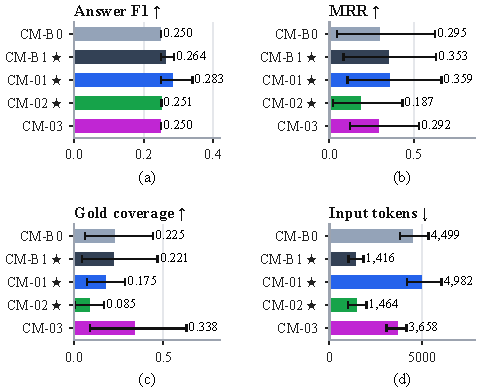
\includegraphics[width=0.96\columnwidth]{figures/fig_rq1_bars.pdf}
\caption{RQ1 per strategy with family-clustered 95\% bootstrap intervals: (a) answer F1, (b) MRR, (c) gold coverage, (d) input tokens. $\bigstar$ marks the Pareto set.}
\label{fig:rq1bars}
\end{figure}

No pair differed significantly in answer F1 (every Holm-adjusted \emph{p}-value was 1.000): all differences came from the two graph-only families. The Pareto set is \{CM-B1, CM-01, CM-02\} (Fig.~\ref{fig:rq1scatter}); CM-B1 dominates CM-B0 and CM-03. By source combination (Fig.~\ref{fig:rq1strata}), correct answers came only from the graph-only families, where CM-01 reached F1 0.384 against 0.307 for CM-B1; on the 18 answerable multi-source questions no strategy returned a correct paper.

\begin{figure}[!t]
\centering
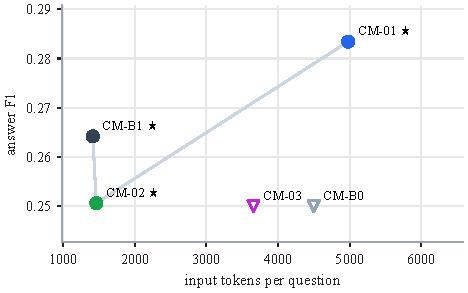
\includegraphics[width=0.91\columnwidth]{figures/fig_rq1_scatter.pdf}
\caption{RQ1 quality against cost. Circles are Pareto-optimal ($\bigstar$), triangles are dominated; up and to the left is better.}
\label{fig:rq1scatter}
\end{figure}

\begin{figure}[!t]
\centering
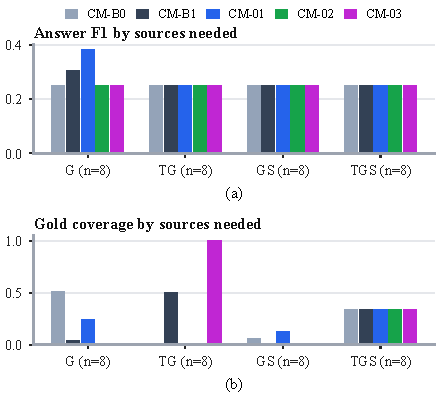
\includegraphics[width=0.94\columnwidth]{figures/fig_rq1_strata.pdf}
\caption{RQ1 by the sources a question needs: (a) answer F1 and (b) gold coverage (8 questions per group). The value 0.25 in (a) is the share of correctly abstained unanswerable variants.}
\label{fig:rq1strata}
\end{figure}

\subsubsection{RQ2: cross-modal fusion}

All five fusion strategies returned an empty answer on all 24 bundles, so answer F1 and exact match are 0.000 for every method (Table~\ref{tab:rq2}). Supportability, fixed before any call, explains most of this (Fig.~\ref{fig:rq2}a): 16 bundles contain no correct paper, 6 contain some, and only 2 contain all; both fully supportable bundles are conflict variants in which the model judged that no paper met every condition. The strategies therefore differ only in cost and ranking. CF-B1 was the cheapest (3,485 input tokens) and fastest (8.4 s) and is the only Pareto-optimal method; CF-02 needed two calls and CF-03 3.75 on average, while CF-03 ranked a correct paper earliest (MRR 0.063). CF-01 resolved every evidence item by its explicit identifier and never needed its registry lookup, and the CF-02 selector kept on average only 0.58 structural items per bundle.

\begin{table}[!t]
\caption{RQ2 cross-modal fusion: means over 24 bundles ($\bigstar$ Pareto-optimal; best in bold)}
\label{tab:rq2}
\centering
\footnotesize
\setlength{\tabcolsep}{3pt}
\renewcommand{\arraystretch}{1.1}
\begin{tabular}{@{}>{\raggedright\arraybackslash}p{\dimexpr0.187\linewidth-2\tabcolsep\relax}>{\raggedleft\arraybackslash}p{\dimexpr0.163\linewidth-2\tabcolsep\relax}>{\raggedleft\arraybackslash}p{\dimexpr0.163\linewidth-2\tabcolsep\relax}>{\raggedleft\arraybackslash}p{\dimexpr0.163\linewidth-2\tabcolsep\relax}>{\raggedleft\arraybackslash}p{\dimexpr0.163\linewidth-2\tabcolsep\relax}>{\raggedleft\arraybackslash}p{\dimexpr0.163\linewidth-2\tabcolsep\relax}@{}}
\toprule
\textbf{Method} & \textbf{F1 $\uparrow$} & \textbf{MRR $\uparrow$} & \textbf{In tok. $\downarrow$} & \textbf{Calls $\downarrow$} & \textbf{Lat. (s) $\downarrow$} \\
\midrule
CF-B0 & 0.000 & 0.029 & 4,097 & \textbf{1.00} & 11.0 \\
CF-B1 $\bigstar$ & 0.000 & 0.029 & \textbf{3,485} & \textbf{1.00} & \textbf{8.4} \\
CF-01 & 0.000 & 0.029 & 4,644 & \textbf{1.00} & 9.1 \\
CF-02 & 0.000 & 0.000 & 3,542 & 2.00 & 12.6 \\
CF-03 & 0.000 & \textbf{0.063} & 4,455 & 3.75 & 19.6 \\
\bottomrule
\end{tabular}
\end{table}

\begin{figure}[!t]
\centering
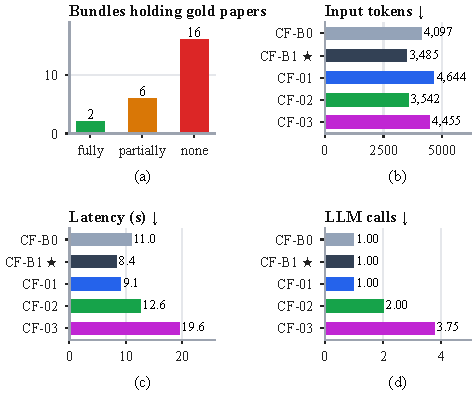
\includegraphics[width=0.96\columnwidth]{figures/fig_rq2.pdf}
\caption{RQ2: (a) supportability of the 24 bundles, fixed before any model call; (b) input tokens, (c) latency, and (d) model calls per bundle.}
\label{fig:rq2}
\end{figure}

No RQ2 difference reached significance. Several cost differences had the same sign in all eight families, e.g., CF-03 used 2.75 more calls per bundle than CF-B1 (unadjusted \emph{p} = 0.008, the minimum attainable with eight families), but with seven pairs per metric their Holm-adjusted \emph{p}-values were at least 0.055 (Section~\ref{sec:discussion}).

\subsubsection{RQ3: retrieval control}

All five policies produced identical answers (F1 0.154, EM 0.143), so efficiency separated them (Table~\ref{tab:rq3}, Fig.~\ref{fig:rq3scatter}). The rule router selected sources best (source F1 0.876) at the lowest cost (1,622 tokens, 8.7 s) and is the only Pareto-optimal policy. Querying every source wasted 43\% of the searches. The agent wasted almost none (0.012) but needed 6.54 model calls per question and was the only policy to miss required sources (0.179).

With 14 families, RQ3 can detect differences (Fig.~\ref{fig:rq3forest}). The router chose sources significantly better than querying everything (+0.176 source F1, Holm-adjusted \emph{p} = 0.014), with significantly less wasted retrieval, fewer searches, fewer tokens ($-$629 per question), and lower latency. Against the router, the learned and agentic policies cost significantly more for the same answers: AR-01 used 2,796 and AR-03 6,096 more tokens per question (both Holm-adjusted \emph{p} = 0.001), and even AR-02 used 283 more (\emph{p} = 0.031); all three were also significantly slower. No policy selected sources significantly better than the router.

\begin{table*}[!t]
\caption{RQ3 retrieval control: means over 28 questions ($\bigstar$ Pareto-optimal; best in bold)}
\label{tab:rq3}
\centering
\footnotesize
\setlength{\tabcolsep}{3pt}
\renewcommand{\arraystretch}{1.1}
\begin{tabular}{@{}>{\raggedright\arraybackslash}p{\dimexpr0.113\linewidth-2\tabcolsep\relax}>{\raggedleft\arraybackslash}p{\dimexpr0.099\linewidth-2\tabcolsep\relax}>{\raggedleft\arraybackslash}p{\dimexpr0.099\linewidth-2\tabcolsep\relax}>{\raggedleft\arraybackslash}p{\dimexpr0.099\linewidth-2\tabcolsep\relax}>{\raggedleft\arraybackslash}p{\dimexpr0.099\linewidth-2\tabcolsep\relax}>{\raggedleft\arraybackslash}p{\dimexpr0.099\linewidth-2\tabcolsep\relax}>{\raggedleft\arraybackslash}p{\dimexpr0.099\linewidth-2\tabcolsep\relax}>{\raggedleft\arraybackslash}p{\dimexpr0.099\linewidth-2\tabcolsep\relax}>{\raggedleft\arraybackslash}p{\dimexpr0.099\linewidth-2\tabcolsep\relax}>{\raggedleft\arraybackslash}p{\dimexpr0.099\linewidth-2\tabcolsep\relax}@{}}
\toprule
\textbf{Method} & \textbf{F1 $\uparrow$} & \textbf{SF1 $\uparrow$} & \textbf{WR $\downarrow$} & \textbf{Stop $\uparrow$} & \textbf{Miss $\downarrow$} & \textbf{Search $\downarrow$} & \textbf{Calls $\downarrow$} & \textbf{Tokens $\downarrow$} & \textbf{Lat. (s) $\downarrow$} \\
\midrule
AR-B0 & 0.154 & 0.700 & 0.429 & \textbf{0.571} & \textbf{0.000} & 3.00 & \textbf{1.00} & 2,251 & 10.6 \\
AR-B1 $\bigstar$ & 0.154 & \textbf{0.876} & 0.190 & \textbf{0.571} & \textbf{0.000} & 2.14 & \textbf{1.00} & \textbf{1,622} & \textbf{8.7} \\
AR-01 & 0.154 & 0.843 & 0.238 & \textbf{0.571} & \textbf{0.000} & 2.43 & 2.71 & 4,419 & 24.1 \\
AR-02 & 0.154 & 0.807 & 0.286 & \textbf{0.571} & \textbf{0.000} & 2.57 & \textbf{1.00} & 1,906 & 10.6 \\
AR-03 & 0.154 & 0.871 & \textbf{0.012} & 0.500 & 0.179 & \textbf{1.86} & 6.54 & 7,719 & 45.2 \\
\bottomrule
\end{tabular}
\end{table*}

\begin{figure}[!t]
\centering
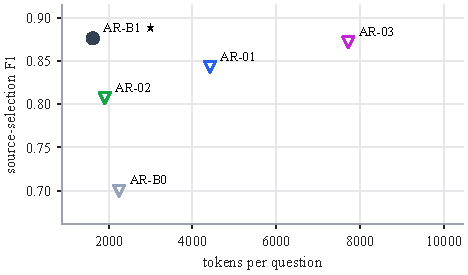
\includegraphics[width=0.91\columnwidth]{figures/fig_rq3_scatter.pdf}
\caption{RQ3 source selection against cost (answer F1 is identical for all policies). AR-B1 is the only Pareto-optimal policy.}
\label{fig:rq3scatter}
\end{figure}

\begin{figure}[!t]
\centering
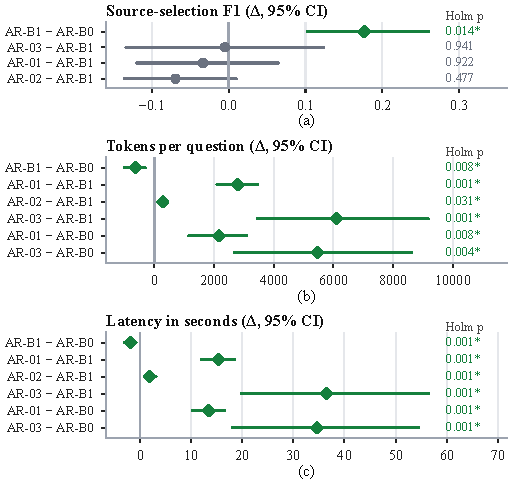
\includegraphics[width=0.96\columnwidth]{figures/fig_rq3_forest.pdf}
\caption{RQ3 paired differences with 95\% family-bootstrap intervals and Holm-adjusted \emph{p}-values (* significant): (a) source-selection F1, (b) tokens, (c) latency.}
\label{fig:rq3forest}
\end{figure}

Fig.~\ref{fig:rq3stops} shows how the policies ended. The classifier of AR-01 chose the multi-step route for every question; its controller judged the evidence sufficient after one search on 8 questions, and the three-search limit ended the other 20. AR-02 rated the evidence GOOD on 6 questions, reached its round limit on 4, and exhausted the sources on 18. The validator of AR-03 accepted a draft answer on 22 questions, 18 of them wrongly, and the iteration limit ended the other 6. A retriever failure despite correct routing was recorded on 24 of the 28 questions for each of AR-B0, AR-B1, AR-01, and AR-02, their joint most frequent failure label; for AR-03 the most frequent label was a false acceptance by the validator.

\begin{figure}[!t]
\centering
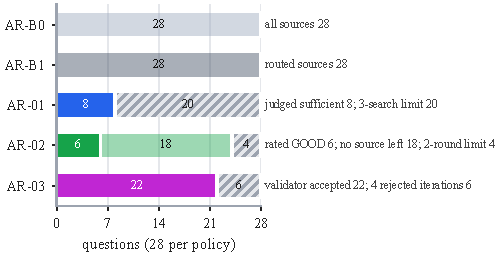
\includegraphics[width=0.97\columnwidth]{figures/fig_rq3_stops.pdf}
\caption{RQ3 stop reasons over the 28 questions: stops decided by the policy (solid), fixed plans completed (light), and limits reached (hatched).}
\label{fig:rq3stops}
\end{figure}

\subsubsection{RQ4: integration}

The frozen rules selected \textbf{AR-B1 $\rightarrow$ CM-B1 $\rightarrow$ CF-B1}. INT-1 gave the same answers as both comparisons (F1 0.154), kept the router's source selection, significantly better than querying everything (+0.176 source F1, Holm-adjusted \emph{p} = 0.004), and used 772 more tokens per question than the router alone (\emph{p} < 0.001), because the CF-B1 fusion stage writes every evidence item as a full record with identifier, payload, and provenance instead of the router's compact lines (7,964 vs. 5,287 context characters on average; Table~\ref{tab:rq4}, Fig.~\ref{fig:rq4}). Latency did not differ significantly. Under the frozen top-5 graph retriever, CM-B1 removed no graph evidence for this single-graph-call policy.

\begin{figure}[!t]
\centering
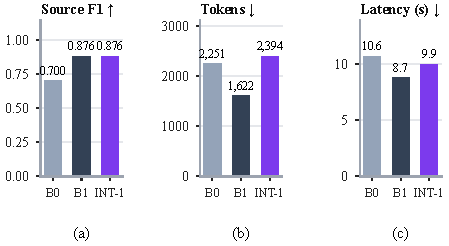
\includegraphics[width=0.94\columnwidth]{figures/fig_rq4.pdf}
\caption{RQ4: (a) source-selection F1, (b) tokens, and (c) latency of AR-B0, AR-B1, and the integrated system INT-1.}
\label{fig:rq4}
\end{figure}

\begin{table}[!t]
\caption{RQ4 integrated system vs. AR-B0 and AR-B1 on 28 questions}
\label{tab:rq4}
\centering
\footnotesize
\setlength{\tabcolsep}{3pt}
\renewcommand{\arraystretch}{1.1}
\begin{tabular}{@{}>{\raggedright\arraybackslash}p{\dimexpr0.187\linewidth-2\tabcolsep\relax}>{\raggedleft\arraybackslash}p{\dimexpr0.163\linewidth-2\tabcolsep\relax}>{\raggedleft\arraybackslash}p{\dimexpr0.163\linewidth-2\tabcolsep\relax}>{\raggedleft\arraybackslash}p{\dimexpr0.163\linewidth-2\tabcolsep\relax}>{\raggedleft\arraybackslash}p{\dimexpr0.163\linewidth-2\tabcolsep\relax}>{\raggedleft\arraybackslash}p{\dimexpr0.163\linewidth-2\tabcolsep\relax}@{}}
\toprule
\textbf{Method} & \textbf{F1 $\uparrow$} & \textbf{SF1 $\uparrow$} & \textbf{Search $\downarrow$} & \textbf{Tokens $\downarrow$} & \textbf{Lat. (s) $\downarrow$} \\
\midrule
AR-B0 & 0.154 & 0.700 & 3.00 & 2,251 & 10.6 \\
AR-B1 & 0.154 & \textbf{0.876} & \textbf{2.14} & \textbf{1,622} & \textbf{8.7} \\
INT-1 & 0.154 & \textbf{0.876} & \textbf{2.14} & 2,394 & 9.9 \\
\bottomrule
\end{tabular}
\end{table}

\subsubsection{Statistical summary}

Table~\ref{tab:sig} lists every difference that survived Holm correction. All of them come from RQ3 and RQ4, whose 14 families give the tests enough resolution.

\begin{table}[!t]
\caption{All paired differences that remain significant after Holm correction (RQ3 and RQ4; $\Delta$ = A $-$ B with family-bootstrap 95\% CI; 14 families)}
\label{tab:sig}
\centering
\footnotesize
\setlength{\tabcolsep}{3pt}
\renewcommand{\arraystretch}{1.1}
\begin{tabular}{@{}>{\raggedright\arraybackslash}p{\dimexpr0.271\linewidth-2\tabcolsep\relax}>{\raggedright\arraybackslash}p{\dimexpr0.177\linewidth-2\tabcolsep\relax}>{\raggedleft\arraybackslash}p{\dimexpr0.149\linewidth-2\tabcolsep\relax}>{\raggedleft\arraybackslash}p{\dimexpr0.266\linewidth-2\tabcolsep\relax}>{\raggedleft\arraybackslash}p{\dimexpr0.137\linewidth-2\tabcolsep\relax}@{}}
\toprule
\textbf{Pair (A $-$ B)} & \textbf{Metric} & \textbf{$\Delta$} & \textbf{95\% CI} & \textbf{\emph{p} (Holm)} \\
\midrule
AR-B1 $-$ AR-B0 & SF1 & +0.176 & [0.102, 0.260] & 0.014 \\
AR-B1 $-$ AR-B0 & WR & $-$0.238 & [$-$0.357, $-$0.131] & 0.012 \\
AR-03 $-$ AR-B0 & WR & $-$0.417 & [$-$0.548, $-$0.286] & 0.003 \\
AR-B1 $-$ AR-B0 & searches & $-$0.86 & [$-$1.21, $-$0.57] & 0.014 \\
AR-03 $-$ AR-B0 & searches & $-$1.14 & [$-$1.64, $-$0.57] & 0.031 \\
AR-B1 $-$ AR-B0 & tokens & $-$629 & [$-$1,010, $-$316] & 0.008 \\
AR-01 $-$ AR-B0 & tokens & +2,168 & [1,162, 3,085] & 0.008 \\
AR-03 $-$ AR-B0 & tokens & +5,467 & [2,684, 8,627] & 0.004 \\
AR-01 $-$ AR-B1 & tokens & +2,796 & [2,101, 3,454] & 0.001 \\
AR-02 $-$ AR-B1 & tokens & +283 & [130, 438] & 0.031 \\
AR-03 $-$ AR-B1 & tokens & +6,096 & [3,447, 9,172] & 0.001 \\
AR-B1 $-$ AR-B0 & latency (s) & $-$1.9 & [$-$3.1, $-$0.8] & 0.001 \\
AR-01 $-$ AR-B0 & latency (s) & +13.4 & [10.2, 16.5] & 0.001 \\
AR-03 $-$ AR-B0 & latency (s) & +34.6 & [18.0, 54.5] & 0.001 \\
AR-01 $-$ AR-B1 & latency (s) & +15.3 & [12.1, 18.4] & 0.001 \\
AR-02 $-$ AR-B1 & latency (s) & +1.8 & [0.8, 3.1] & 0.001 \\
AR-03 $-$ AR-B1 & latency (s) & +36.5 & [19.8, 56.4] & 0.001 \\
INT-1 $-$ AR-B0 & SF1 & +0.176 & [0.102, 0.260] & 0.004 \\
INT-1 $-$ AR-B1 & tokens & +772 & [596, 946] & < 0.001 \\
\bottomrule
\end{tabular}
\end{table}

No answer-quality difference is among them: every significant difference concerns source selection or cost.

\begin{table}[!t]
\caption{Overall winners (rank totals over the Pareto axes; lower is better)}
\label{tab:rank}
\centering
\footnotesize
\setlength{\tabcolsep}{3pt}
\renewcommand{\arraystretch}{1.1}
\begin{tabular}{@{}>{\raggedright\arraybackslash}p{\dimexpr0.132\linewidth-2\tabcolsep\relax}>{\raggedright\arraybackslash}p{\dimexpr0.250\linewidth-2\tabcolsep\relax}>{\raggedright\arraybackslash}p{\dimexpr0.263\linewidth-2\tabcolsep\relax}>{\raggedright\arraybackslash}p{\dimexpr0.197\linewidth-2\tabcolsep\relax}>{\raggedright\arraybackslash}p{\dimexpr0.158\linewidth-2\tabcolsep\relax}@{}}
\toprule
\textbf{Study} & \textbf{Winner} & \textbf{Runner-up} & \textbf{Scaled check} & \textbf{Quality-first} \\
\midrule
RQ1 & CM-B1 (7) & CM-01, CM-02 (11) & CM-B1 (0.838) & CM-01 \\
RQ2 & CF-B1 (5) & CF-02, CF-B0 (9) & CF-B1 (1.000) & CF-B1 \\
RQ3 & AR-B1 (6) & AR-02 (11) & AR-B1 (1.000) & AR-B1 \\
\bottomrule
\end{tabular}
\end{table}

\subsubsection{Overall ranking}

Table~\ref{tab:rank} and Fig.~\ref{fig:ranking} report the overall ranking. CM-B1 wins RQ1 with a rank total of 7 (second on F1, MRR, and latency, first on tokens), CF-B1 wins RQ2 (5; first on both cost axes with F1 tied), and AR-B1 wins RQ3 (6; first on source F1, tokens, and latency). The scaled-score check selects the same winner in every study. Chained in pipeline order, the winners are exactly INT-1, which the frozen rule had selected before the ranking was defined. A quality-first rule would choose CM-01 in RQ1 and the same winners elsewhere.

\begin{figure}[!t]
\centering
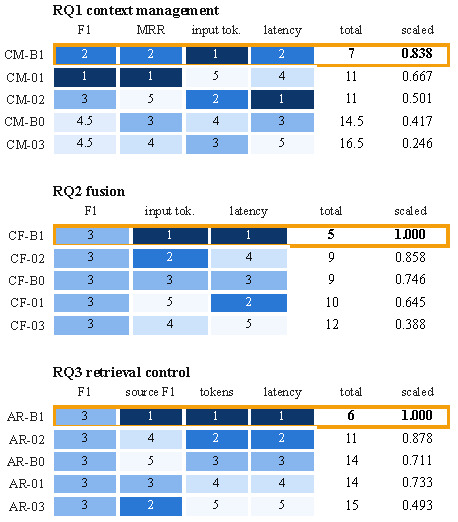
\includegraphics[width=0.94\columnwidth]{figures/fig_ranking.pdf}
\caption{Overall ranking per study: rank on each Pareto axis (1 = best; darker is better), rank total, and scaled score. The outlined row is the winner.}
\label{fig:ranking}
\end{figure}

\subsection{Discussion}\label{sec:discussion}

\subsubsection{Why the simplest strategies win}

Three effects combine. First, answers did not separate the strategies: in RQ1 no difference was significant (and, as shown below, none could be), and in RQ2--RQ4 every strategy returned identical answers, so cost and evidence selection decided the ranking. Second, the elaborate methods act after retrieval: rerankers, Steiner trees, diffusion, entity alignment, model-based selection, per-source reasoning, trained routers, calibrated evaluators, and agents all reorganize evidence that the retrievers already returned and cannot recover correct papers that were never retrieved, yet they add model calls, tokens, and time. Third, the controls are well matched to the questions: the rule router benefits from cue words in templated questions, and the fixed top-K follows the retriever's own ranking. These findings concern this corpus, these retrievers, and this model; they do not show that the elaborate mechanisms are ineffective in general.

\subsubsection{Where answer quality is lost}

Fig.~\ref{fig:bottleneck} locates the loss before generation. In a retrieval-only check of the four baselines on 56 validation questions, the structured retriever found every correct paper of structured-only questions and a third of those of three-source questions, the graph retriever found 4\% of the correct papers of graph-only questions, and the dense text retriever found almost none (0.003 on text-only questions), because text conditions are exact phrases while the retriever searches by meaning; no retriever found a correct paper of any text-and-graph question. Consequently, in RQ3 every policy answered the structured-only questions exactly (F1 1.000), the graph-only questions weakly (0.076, since a top-5 holds few of their many correct papers), and no other combination at all; the overall F1 of 0.154 is exactly this mixture. The same pattern bounds RQ1 (gold coverage of at most 0.338) and RQ2 (16 unsupportable bundles). Even where the correct paper was present, the model abstained when it could not verify every condition, which is the behaviour the grounding prompt requests.

\begin{figure}[!t]
\centering
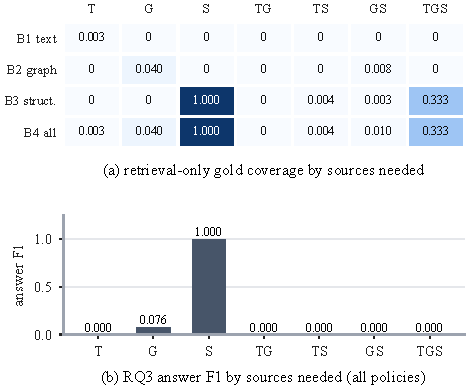
\includegraphics[width=0.94\columnwidth]{figures/fig_bottleneck.pdf}
\caption{Where answer quality is lost: (a) retrieval-only gold coverage of the four baselines by the sources a question needs (56 validation questions); (b) answer F1 of every RQ3 policy by the sources a question needs (4 questions per group).}
\label{fig:bottleneck}
\end{figure}

\begin{table}[!t]
\caption{Situations in which another strategy measured better (descriptive)}
\label{tab:situations}
\centering
\footnotesize
\setlength{\tabcolsep}{3pt}
\renewcommand{\arraystretch}{1.1}
\begin{tabular}{@{}>{\raggedright\arraybackslash}p{\dimexpr0.119\linewidth-2\tabcolsep\relax}>{\raggedright\arraybackslash}p{\dimexpr0.327\linewidth-2\tabcolsep\relax}>{\raggedright\arraybackslash}p{\dimexpr0.156\linewidth-2\tabcolsep\relax}>{\raggedright\arraybackslash}p{\dimexpr0.398\linewidth-2\tabcolsep\relax}@{}}
\toprule
\textbf{Study} & \textbf{Situation} & \textbf{Pick} & \textbf{Evidence} \\
\midrule
RQ1 & answer quality matters more than cost & CM-01 & F1 0.283, MRR 0.359; 3.5$\times$ tokens \\
RQ1 & every correct paper must reach the model & CM-03 & GC 0.338; slowest (40.7 s) \\
RQ1 & speed is the priority & CM-02 & 6.5 s; lowest MRR \\
RQ2 & a correct paper should rank early & CF-03 & MRR 0.063 vs. 0.029; 3.75 calls \\
RQ2 & exactly two sources needed & CF-02 & fewest tokens on TG, TS, and GS bundles \\
RQ3 & each search is expensive & AR-03 & WR 0.012 vs. 0.190 \\
RQ3 & text-only questions & AR-03 & SF1 1.000 vs. 0.667 \\
RQ3 & graph-only questions & AR-01 & SF1 1.000 vs. 0.667 \\
\bottomrule
\end{tabular}
\end{table}

\subsubsection{When another strategy is preferable}

The winners are the best overall choice, but in specific situations another strategy measured better (Table~\ref{tab:situations}). These group-level differences are descriptive (4--8 questions per group) and were not tested.

\subsubsection{Statistical power}

The exact sign-flip test cannot return a \emph{p}-value below $2/2^F$. With $F=8$ families this floor is 0.0078, and Holm multiplies the smallest \emph{p}-value by the number of pairs, so the smallest attainable adjusted \emph{p}-values were $10\times 0.0078=0.078$ in RQ1 and $7\times 0.0078=0.055$ in RQ2, both above 0.05. No difference in RQ1 or RQ2 could have been declared significant however consistent it was; their conclusions rest on the means and on consistency across families. With 14 families, RQ3 and RQ4 could detect differences and did. Future studies should either use more families or pre-specify fewer pairs.

\subsubsection{Implications for practice}

Four guidelines follow. (i) Measure upstream coverage (gold coverage, supportability) before optimizing downstream components; no downstream method recovered what retrieval missed. (ii) Treat simple controls as strong baselines and always report cost: a fixed top-K, labelled sections, and keyword routing matched the elaborate methods' answers at a fraction of their cost. (iii) Match the retriever to the condition type: exact phrases call for lexical or hybrid text retrieval. (iv) Make experiments replayable: storing every request by its hash made multi-day runs resumable and every number auditable.

\subsubsection{Threats to validity}

\emph{Internal validity} is protected by freezing, identical inputs, question-major call order, and replay verification; a recorded timing asymmetry slightly favours CM-02 and CM-03 in latency, because their query-specific scores were staged offline while CM-01 computes them inside its timer. \emph{Construct validity}: answer F1 against verified sets is exact, but gold coverage is an upper bound rather than accuracy, and template wording flatters the rule router. \emph{External validity}: one corpus, three simple retrievers, and one model; the methods are adaptations, not reproductions. \emph{Statistical conclusion validity}: small cohorts of correlated variants, analysed at the family level as described above.

\section{Conclusion}\label{sec:conclusion}

This paper studied, one component at a time, how a retrieval-augmented LLM should use text, graph, and structured views of the same scholarly corpus. On isolated, identity-joined views and a benchmark with verified source necessity, under frozen retrievers and one LLM, one strategy won each component on combined quality and cost: fixed top-K context management (CM-B1), source-separated fusion (CF-B1), and rule-based routing (AR-B1). Their combination, INT-1, which the pre-registered rule had already selected, answered as well as any single policy (F1 0.154), selected sources significantly better than querying every source (+0.176 source F1), and used 772 more tokens per question than the router alone. No literature-inspired method improved answer quality with statistical support, and the most elaborate controllers cost significantly more. The clearest lesson is where quality is lost: before generation, in retrieval coverage.

\subsection{Limitations and Future Work}

\textbf{Limitations.} The cohorts are small (8--14 independent families), so the results are exploratory validation results rather than a locked test, and in RQ1 and RQ2 significance was unattainable. Labels are verified by computation; human review of the test sets (2,801 decisions) is outstanding. Text conditions are exact phrases that a meaning-based retriever rarely finds, and template wording favours the rule router. One corpus, one set of simple retrievers, and one LLM were used. All literature methods are adaptations: training-heavy components of the originals were replaced or omitted, CM-01 uses graph-native provenance units, and CM-03 converged on few questions under its frozen parameters. Under the frozen top-5 graph retriever, CM-B1 prunes only for policies with several graph calls.

\textbf{Future work.} (i) Raise upstream coverage with lexical or hybrid text retrieval, adaptive graph top-K, and structured filters that restrict candidates for the other sources, then repeat the component studies where answers are possible. (ii) Complete the human review and run the locked test. (iii) Repeat the comparisons with a stronger LLM and larger budgets. (iv) Evaluate fusion on evidence-complete bundles. (v) Increase statistical power with more families and fewer pre-specified pairs. (vi) Test on natural, human-written multi-source questions with verified source necessity.

\section{Dataset and Code Availability}\label{sec:availability}

\subsection{Dataset}

All experiments use the official STaRK-MAG release~\cite{wu2024stark,wang2020mag}:

\begin{itemize}
\item \textbf{Source:} \url{https://huggingface.co/datasets/snap-stanford/stark}
\item \textbf{Revision:} 88269e23e90587f99476c5dd74e235a0877e69be
\item \textbf{Licence:} CC-BY-4.0, as recorded on the dataset card.
\end{itemize}

The three views of MMG-STaRK-MAG and the benchmark are derived deterministically from this release by the released build scripts and are verified against recorded SHA-256 manifests (benchmark manifest e07f1314\ldots{}). No human-review decisions are released, and the test and human-test splits were never used.

\subsection{Code Availability}

The complete code will be released on GitHub (link to be added):

\begin{itemize}
\item \textbf{Repository:} \url{https://github.com/[account]/[repository]}
\end{itemize}

It contains the data build, benchmark construction, retrievers, all strategies, the execution protocol, the analyses, the generators of every figure and table in this paper, and an interactive showcase application with the recorded runs. Each study is accompanied by its frozen execution plan, stored model requests, run records, and analysis files, so every number can be rebuilt without calling the model again.

\begin{thebibliography}{00}
\bibitem{lewis2020} P. Lewis \emph{et al.}, ``Retrieval-augmented generation for knowledge-intensive NLP tasks,'' in \emph{Proc. Adv. Neural Inf. Process. Syst. (NeurIPS)}, 2020, pp. 9459--9474.
\bibitem{gao2023} Y. Gao \emph{et al.}, ``Retrieval-augmented generation for large language models: A survey,'' 2023, \emph{arXiv:2312.10997}.
\bibitem{he2024gretriever} X. He \emph{et al.}, ``G-Retriever: Retrieval-augmented generation for textual graph understanding and question answering,'' in \emph{Proc. Adv. Neural Inf. Process. Syst. (NeurIPS)}, 2024.
\bibitem{zhu2025kg2rag} X. Zhu, Y. Xie, Y. Liu, Y. Li, and W. Hu, ``Knowledge graph-guided retrieval augmented generation,'' 2025, \emph{arXiv:2502.06864}.
\bibitem{zhou2026qafd} Z. Zhou \emph{et al.}, ``Query-aware flow diffusion for graph-based RAG with retrieval guarantees,'' in \emph{Proc. Int. Conf. Learn. Represent. (ICLR)}, 2026.
\bibitem{liang2024kag} L. Liang \emph{et al.}, ``KAG: Boosting LLMs in professional domains via knowledge augmented generation,'' 2024, \emph{arXiv:2409.13731}.
\bibitem{wu2026sag} Y. Wu \emph{et al.}, ``SAG: SQL-retrieval augmented generation with query-time dynamic hyperedges,'' 2026, \emph{arXiv:2606.15971}.
\bibitem{hsiao2025megarag} C.-H. Hsiao, Y.-C. Wang, T.-S. Lin, Y.-R. Yeh, and C.-S. Chen, ``MegaRAG: Multimodal knowledge graph-based retrieval augmented generation,'' 2025, \emph{arXiv:2512.20626}.
\bibitem{jeong2024adaptive} S. Jeong, J. Baek, S. Cho, S. J. Hwang, and J. C. Park, ``Adaptive-RAG: Learning to adapt retrieval-augmented large language models through question complexity,'' in \emph{Proc. Conf. North Amer. Chapter Assoc. Comput. Linguistics (NAACL)}, 2024.
\bibitem{yan2024crag} S.-Q. Yan, J.-C. Gu, Y. Zhu, and Z.-H. Ling, ``Corrective retrieval augmented generation,'' 2024, \emph{arXiv:2401.15884}.
\bibitem{agentg2025} Anonymous, ``AGENT-G: An agentic framework for graph retrieval augmented generation,'' submitted to \emph{Int. Conf. Learn. Represent. (ICLR)}, OpenReview, 2024. [Online]. Available: \url{https://openreview.net/forum?id=g2C947jjjQ}
\bibitem{holm1979} S. Holm, ``A simple sequentially rejective multiple test procedure,'' \emph{Scand. J. Statist.}, vol. 6, no. 2, pp. 65--70, 1979.
\bibitem{efron1993} B. Efron and R. J. Tibshirani, \emph{An Introduction to the Bootstrap}. New York, NY, USA: Chapman \& Hall, 1993.
\bibitem{cameron2008} A. C. Cameron, J. B. Gelbach, and D. L. Miller, ``Bootstrap-based improvements for inference with clustered errors,'' \emph{Rev. Econ. Statist.}, vol. 90, no. 3, pp. 414--427, 2008.
\bibitem{liu2024lost} N. F. Liu \emph{et al.}, ``Lost in the middle: How language models use long contexts,'' \emph{Trans. Assoc. Comput. Linguistics}, vol. 12, pp. 157--173, 2024.
\bibitem{jiang2024longllmlingua} H. Jiang \emph{et al.}, ``LongLLMLingua: Accelerating and enhancing LLMs in long context scenarios via prompt compression,'' in \emph{Proc. Annu. Meeting Assoc. Comput. Linguistics (ACL)}, 2024.
\bibitem{jiang2023flare} Z. Jiang \emph{et al.}, ``Active retrieval augmented generation,'' in \emph{Proc. Conf. Empirical Methods Natural Lang. Process. (EMNLP)}, 2023, pp. 7969--7992.
\bibitem{asai2024selfrag} A. Asai, Z. Wu, Y. Wang, A. Sil, and H. Hajishirzi, ``Self-RAG: Learning to retrieve, generate, and critique through self-reflection,'' in \emph{Proc. Int. Conf. Learn. Represent. (ICLR)}, 2024.
\bibitem{edge2024graphrag} D. Edge \emph{et al.}, ``From local to global: A graph RAG approach to query-focused summarization,'' 2024, \emph{arXiv:2404.16130}.
\bibitem{goemans1995} M. X. Goemans and D. P. Williamson, ``A general approximation technique for constrained forest problems,'' \emph{SIAM J. Comput.}, vol. 24, no. 2, pp. 296--317, 1995.
\bibitem{hegde2015pcst} C. Hegde, P. Indyk, and L. Schmidt, ``A nearly-linear time framework for graph-structured sparsity,'' in \emph{Proc. Int. Conf. Mach. Learn. (ICML)}, 2015, pp. 928--937.
\bibitem{fountoulakis2020flow} K. Fountoulakis, D. Wang, and S. Yang, ``p-Norm flow diffusion for local graph clustering,'' in \emph{Proc. Int. Conf. Mach. Learn. (ICML)}, 2020, pp. 3222--3232.
\bibitem{sun2024tog} J. Sun \emph{et al.}, ``Think-on-Graph: Deep and responsible reasoning of large language model on knowledge graph,'' in \emph{Proc. Int. Conf. Learn. Represent. (ICLR)}, 2024.
\bibitem{gutierrez2024hipporag} B. J. Gutiérrez, Y. Shu, Y. Gu, M. Yasunaga, and Y. Su, ``HippoRAG: Neurobiologically inspired long-term memory for large language models,'' in \emph{Proc. Adv. Neural Inf. Process. Syst. (NeurIPS)}, 2024.
\bibitem{peng2024survey} B. Peng \emph{et al.}, ``Graph retrieval-augmented generation: A survey,'' 2024, \emph{arXiv:2408.08921}.
\bibitem{oguz2022unikqa} B. Oguz \emph{et al.}, ``UniK-QA: Unified representations of structured and unstructured knowledge for open-domain question answering,'' in \emph{Findings Assoc. Comput. Linguistics: NAACL}, 2022, pp. 1535--1546.
\bibitem{jiang2023structgpt} J. Jiang, K. Zhou, Z. Dong, K. Ye, W. X. Zhao, and J.-R. Wen, ``StructGPT: A general framework for large language model to reason over structured data,'' in \emph{Proc. Conf. Empirical Methods Natural Lang. Process. (EMNLP)}, 2023, pp. 9237--9251.
\bibitem{sarmah2024hybridrag} B. Sarmah, B. Hall, R. Rao, S. Patel, S. Pasquali, and D. Mehta, ``HybridRAG: Integrating knowledge graphs and vector retrieval augmented generation for efficient information extraction,'' in \emph{Proc. ACM Int. Conf. AI Finance (ICAIF)}, 2024.
\bibitem{bu2025qdmm} C. Bu \emph{et al.}, ``Query-driven multimodal GraphRAG: Dynamic local knowledge graph construction for online reasoning,'' in \emph{Findings Assoc. Comput. Linguistics: ACL}, 2025, pp. 21360--21380.
\bibitem{trivedi2023ircot} H. Trivedi, N. Balasubramanian, T. Khot, and A. Sabharwal, ``Interleaving retrieval with chain-of-thought reasoning for knowledge-intensive multi-step questions,'' in \emph{Proc. Annu. Meeting Assoc. Comput. Linguistics (ACL)}, 2023, pp. 10014--10037.
\bibitem{yao2023react} S. Yao \emph{et al.}, ``ReAct: Synergizing reasoning and acting in language models,'' in \emph{Proc. Int. Conf. Learn. Represent. (ICLR)}, 2023.
\bibitem{maharjan2026agent} A. Maharjan, D. Kaur, and R. G. Molyet, ``Agent-orchestrated adaptive RAG: A comparative study on structured and multi-hop retrieval,'' 2026, \emph{arXiv:2606.05658}.
\bibitem{wu2024stark} S. Wu \emph{et al.}, ``STaRK: Benchmarking LLM retrieval on textual and relational knowledge bases,'' in \emph{Proc. Adv. Neural Inf. Process. Syst. (NeurIPS), Datasets Benchmarks Track}, 2024.
\bibitem{wang2020mag} K. Wang, Z. Shen, C. Huang, C.-H. Wu, Y. Dong, and A. Kanakia, ``Microsoft Academic Graph: When experts are not enough,'' \emph{Quant. Sci. Stud.}, vol. 1, no. 1, pp. 396--413, 2020.
\bibitem{dror2018} R. Dror, G. Baumer, S. Shlomov, and R. Reichart, ``The hitchhiker's guide to testing statistical significance in natural language processing,'' in \emph{Proc. Annu. Meeting Assoc. Comput. Linguistics (ACL)}, 2018, pp. 1383--1392.
\bibitem{good2005} P. Good, \emph{Permutation, Parametric, and Bootstrap Tests of Hypotheses}, 3rd ed. New York, NY, USA: Springer, 2005.
\bibitem{reimers2019sbert} N. Reimers and I. Gurevych, ``Sentence-BERT: Sentence embeddings using Siamese BERT-networks,'' in \emph{Proc. Conf. Empirical Methods Natural Lang. Process. Int. Joint Conf. Natural Lang. Process. (EMNLP-IJCNLP)}, 2019, pp. 3982--3992.
\bibitem{wang2020minilm} W. Wang, F. Wei, L. Dong, H. Bao, N. Yang, and M. Zhou, ``MiniLM: Deep self-attention distillation for task-agnostic compression of pre-trained transformers,'' in \emph{Proc. Adv. Neural Inf. Process. Syst. (NeurIPS)}, 2020.
\bibitem{johnson2021faiss} J. Johnson, M. Douze, and H. Jégou, ``Billion-scale similarity search with GPUs,'' \emph{IEEE Trans. Big Data}, vol. 7, no. 3, pp. 535--547, Jul. 2021.
\bibitem{raasveldt2019duckdb} M. Raasveldt and H. Mühleisen, ``DuckDB: An embeddable analytical database,'' in \emph{Proc. ACM SIGMOD Int. Conf. Manage. Data}, 2019, pp. 1981--1984.
\bibitem{openai2025gptoss} OpenAI, ``gpt-oss-120b \& gpt-oss-20b model card,'' 2025, \emph{arXiv:2508.10925}.
\bibitem{ollama} Ollama, ``Ollama: Get up and running with large language models locally,'' 2025. [Online]. Available: \url{https://ollama.com}
\bibitem{kruskal1956} J. B. Kruskal, ``On the shortest spanning subtree of a graph and the traveling salesman problem,'' \emph{Proc. Amer. Math. Soc.}, vol. 7, no. 1, pp. 48--50, 1956.
\bibitem{xiao2024cpack} S. Xiao, Z. Liu, P. Zhang, N. Muennighoff, D. Lian, and J.-Y. Nie, ``C-Pack: Packed resources for general Chinese embeddings,'' in \emph{Proc. Int. ACM SIGIR Conf. Res. Develop. Inf. Retrieval (SIGIR)}, 2024.
\bibitem{raffel2020t5} C. Raffel \emph{et al.}, ``Exploring the limits of transfer learning with a unified text-to-text transformer,'' \emph{J. Mach. Learn. Res.}, vol. 21, no. 140, pp. 1--67, 2020.
\bibitem{nogueira2019monobert} R. Nogueira and K. Cho, ``Passage re-ranking with BERT,'' 2019, \emph{arXiv:1901.04085}.
\bibitem{bajaj2016msmarco} P. Bajaj \emph{et al.}, ``MS MARCO: A human generated machine reading comprehension dataset,'' 2016, \emph{arXiv:1611.09268}.
\bibitem{platt1999} J. C. Platt, ``Probabilistic outputs for support vector machines and comparisons to regularized likelihood methods,'' in \emph{Advances in Large Margin Classifiers}, A. J. Smola, P. Bartlett, B. Schölkopf, and D. Schuurmans, Eds. Cambridge, MA, USA: MIT Press, 1999, pp. 61--74.
\end{thebibliography}

\end{document}
